% ANIMA Phase I white paper — main file.
% Compile: tectonic main.tex (or pdflatex+bibtex+pdflatex x2).
\documentclass[11pt]{article}

\usepackage[margin=1.05in]{geometry}
\usepackage{amsmath,amssymb}
\usepackage{booktabs}
\usepackage{graphicx}
\usepackage{xcolor}
\usepackage{tikz}
\usetikzlibrary{arrows.meta,positioning,shapes.geometric}
\usepackage{caption}
\usepackage{enumitem}
\usepackage[hidelinks]{hyperref}

\definecolor{established}{RGB}{23,120,53}
\definecolor{supported}{RGB}{50,130,200}
\definecolor{partial}{RGB}{220,150,20}
\definecolor{notest}{RGB}{180,40,40}
\definecolor{cEst}{RGB}{23,120,53}
\definecolor{cDem}{RGB}{50,130,200}
\definecolor{cPar}{RGB}{220,150,20}
\definecolor{cNo}{RGB}{180,40,40}
\emergencystretch=2em

\title{\bfseries ANIMA Phase I: Emergent Organization and the\\ Architectural Limits of Persistent Learning in a\\ Minimally Specified Spiking Nervous System}
\author{ANIMA project \\ Experimental developmental artificial nervous system --- Phase I record}
\date{September 2026}

\begin{document}
\maketitle

\begin{abstract}
ANIMA is an experimental developmental artificial nervous system: a
deterministically seeded spiking substrate in which only the boundaries
--- sensory input, output, environment, curriculum, resource limits,
and local plasticity laws --- are specified, and nothing else. Phase I
asked whether useful, stable, adaptive internal organization can arise
from such a minimal specification, and progressed through a series of
frozen, identity-gated experiments to locate the architectural limit of
persistent learning. The record demonstrates, in turn: sensory-specific
synaptic organization emerges from spike-timing-dependent plasticity
under purely local rules; transient spike-based representations exist
during stimulation; scalar intrinsic persistence is information-poor
and cannot serve as sensory memory; the synaptic weight structure is
the substrate's persistent store, but it suffers order-dependent
interference --- blocked sequential experience overwrites, alternated
experience superposes; bounded consolidation protects the store from
runaway and preserves alternating coexistence; and, once stability was
established, the limiting factor moved successively to allocation, to
first-exposure allocation, and finally to the recruitment of postsynaptic
activity for genuinely novel late-arriving patterns, which Phase I
leaves unresolved. Throughout, the project enforced pre-registered
protocols, byte-identical flag-off control gates, deterministic replay,
and preservation of negative results, so that each negative narrows the
space of possible architectures rather than being discarded. The paper
reports what is demonstrated, what is supported, what is unmeasured,
and what remains hypothesis, with every quantitative claim traceable to
a committed repository record.
\end{abstract}

\parbox{\textwidth}{\raggedright\textbf{Keywords:} emergent organization; spiking neural substrate; persistent synaptic structure; synaptic interference; allocation; identity discipline; pre-registration; minimal specification.}\par\medskip

\tableofcontents

\section{Introduction}\label{sec:intro}
Biological nervous systems are not engineered as circuits; they develop.
A research program that takes development seriously therefore faces a
choice of specification: prescribe the final organization (a designed
network), or prescribe only the materials and the laws and ask whether
organization arises. The ANIMA project takes the second path. Its
charter fixes only the sensory boundary, the output boundary, the
environment and curriculum, finite resource limits, and fundamental
local plasticity laws, and requires that the organism --- a population
of spiking neurons --- develop useful, stable, adaptive internal
organization through interaction, without any prescription of the final
organization \cite{overview,decisionlog}.

Three commitments follow from this framing and structure everything
reported here. First, \emph{minimal specification}: no task-specific
semantic variables, no labels, no reward or credit assignment, no
hidden supervision, and no hand-designed internal architecture. The
organism's ``concepts'' are whatever its plasticity laws and its
curriculum make of its inputs. Second, \emph{locality}: all mechanisms
operate on local state --- membrane potentials, arriving currents,
synaptic weights, and per-neuron budgets. Third, \emph{determinism and
discipline}: every experiment is frozen in writing before
implementation, runs under a single seeded random number generator so
that same-seed reproduction is byte-identical, is gated by a
flag-off identity check against the committed baseline, and preserves
its negative results \cite{overview}.

The research question of Phase I is deliberately modest in form and
demanding in content:

\begin{quote}
\emph{In a minimally specified spiking substrate with local plasticity
and finite resources, what internal organization emerges, what of it
persists, and what are the architectural limits of persistent,
retrievable learning under sequential experience?}
\end{quote}

The answer, as measured rather than assumed, is summarized by the
progression in Figure~\ref{fig:architecture} and developed through the
rest of the paper. The phrase ``architectural limits'' is used
advisedly: Phase I's contribution is not a system that works, but a
map of the causal chain through which each candidate substrate failed,
with the failure point identified at each step. The final step ---
recruiting postsynaptic activity for a genuinely novel pattern that
arrives late in a blocked curriculum --- is a measurement of where the
current architecture stops, not a claim that the class of architectures
is exhausted.

\subsection{Relation to related work}

The substrate is an orthodox leaky-integrate-and-fire (LIF) population
with pairwise additive spike-timing-dependent plasticity (STDP)
\cite{gerstner2002,bipoo1998}. The aspiration --- that competitive
Hebbian learning organizes selective assemblies --- has a long
theoretical lineage \cite{hebb1949,song2000}. ANIMA differs from that
lineage in its discipline rather than its ingredients: organization is
never scored by a task the experimenter cares about; the curriculum is
a fixed, deterministic schedule of synthetic pattern presentations; and
every mechanism claim is tested under flag-off byte-identity control.
The value of the record is therefore mostly negative: it shows, under
these controls, exactly which attractive properties of the ingredients
fail to materialize, and where successive local amendments move the
failure.

\section{Design Philosophy}\label{sec:philosophy}
The operating constraints that shaped every experiment are documented
in the charter and decision log \cite{overview,decisionlog}. They are
restated here because they are load-bearing for the interpretation of
every result.

\paragraph{Specified interfaces, not architectures.}
The project defines the sensory front end (input channels with
deterministic Poisson spike trains per presentation), the output
boundary (ordinary plastic neurons whose spikes are additionally
emitted as output activity --- a role tag, not a cell type), the
environment/curriculum (an ordered schedule of pattern presentations),
resource limits (neuron, synapse, per-neuron budget caps), and the
plasticity laws (STDP, weight normalization, candidate/prune machinery,
anti-Hebbian inhibition). It never defines assemblies, readout circuits,
or any intermediate organization.

\paragraph{Local rules.}
Every mechanism is required to read only per-neuron or per-synapse
state. This is enforced loosely in design and strictly at review: the
CLLA falsifier F5 requires static conformance --- consolidation and
allocation decision paths may not read pattern identity, channel-group
membership tests, presentation counts, or any global state
\cite{cllaprot,cllarecord}.

\paragraph{Finite resources.}
A neuron owns a total excitatory budget \(t_e = 0.8\) (weight units, M2
normalization) and a candidate pool of six slots; consolidation may
protect at most \(p_{\max} t_e = 0.60\) of the budget; budgets bind
synapse creation (M5, \(b_e = 40\) excitatory afferents per neuron).
Resource limits are treated as part of the specification, not as an
implementation nuisance.

\paragraph{No semantic supervision.}
All presented patterns are examples; the curriculum is a configurable
schedule, not a set of preinstalled concepts. The organism is never told
which pattern it is seeing, whether a response was correct, or that a
pattern is ``novel.''

\paragraph{Reproducibility and freeze discipline.}
Protocols are committed before implementation; amendments are logged
and user-approved; every execution is byte-deterministic under a seeded
Xoshiro generator; a flag-off ``identity gate'' must reproduce the
committed baseline byte-for-byte (event-stream hash and snapshot
frames) before any flag-on run is interpreted; and negative results are
preserved with their runs \cite{overview,cllaprot}. Several protocol
defects were discovered only by this discipline and are reported as
such (\S\ref{sec:clla}, \S\ref{sec:method}).

\begin{figure}[t]
\centering
\resizebox{\textwidth}{!}{%
% Figure 1 — ANIMA architecture + experimental philosophy (schematic).
% Every annotation in the right panel is established in the cited records.
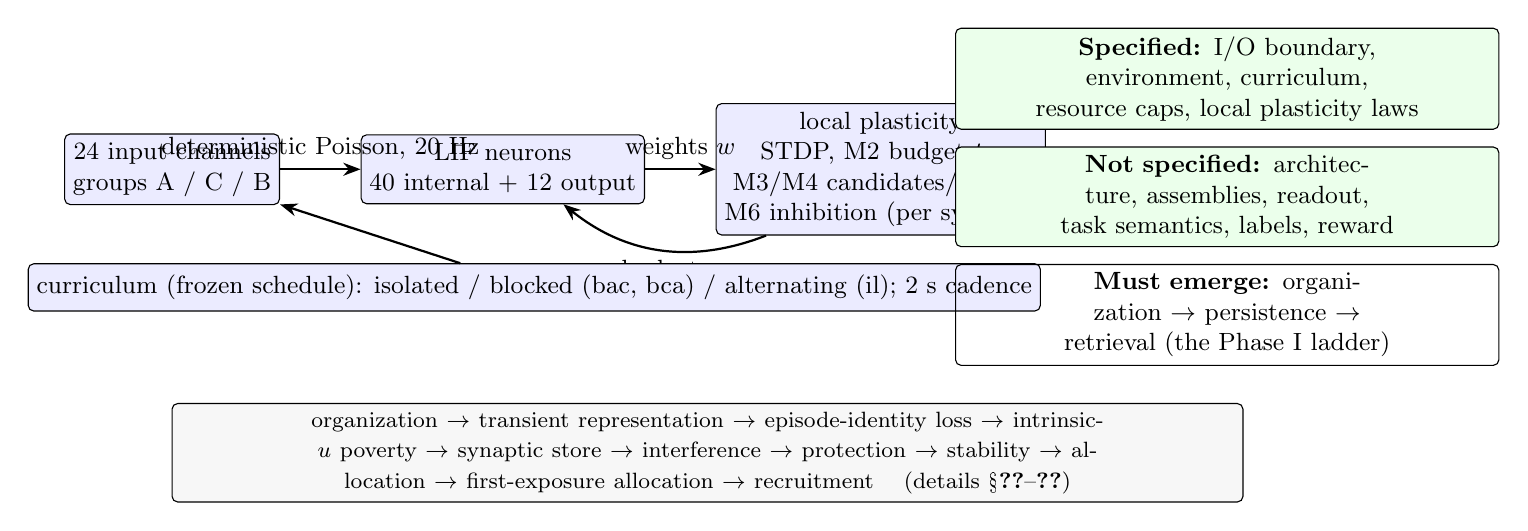
\begin{tikzpicture}[
  box/.style={draw, rounded corners=2pt, minimum height=6mm, font=\small,
              align=center, inner sep=3pt},
  spec/.style={fill=blue!8}, emerge/.style={fill=green!8},
  arrow/.style={-{Stealth[length=2.2mm]}, thick}
]
  % layer 1: input
  \node[box, spec] (inp) at (0, 0) {24 input channels\\groups A / C / B};
  % layer 2: network
  \node[box, spec] (net) at (4.2, 0) {LIF neurons\\40 internal + 12 output};
  % layer 3: plasticity (box to the right)
  \node[box, spec, minimum width=3.2cm] (plast) at (9.0, 0) {local plasticity\\STDP, M2 budget $t_e$,\\M3/M4 candidates/prune,\\M6 inhibition (per synapse)};
  \draw[arrow] (inp) -- node[above, font=\small] {deterministic Poisson, 20 Hz} (net);
  \draw[arrow] (net) -- node[above, font=\small] {weights $w$} (plast);
  \draw[arrow] (plast) to[bend left=30] node[below, font=\small] {budget} (net);
  % environment / curriculum
  \node[box, spec, minimum width=8.9cm] (env) at (4.6, -1.5) {curriculum (frozen schedule): isolated / blocked (bac, bca) / alternating (il); 2 s cadence};
  \draw[arrow] (env) -- (inp);

  % right panel: philosophy
  \node[box, emerge, font=\small, minimum width=6.9cm, text width=6.5cm] (p1) at (13.4, 1.15)
    {\textbf{Specified:} I/O boundary, environment, curriculum,\\resource caps, local plasticity laws};
  \node[box, emerge, font=\small, minimum width=6.9cm, text width=6.5cm] (p2) at (13.4, -0.35)
    {\textbf{Not specified:} architecture, assemblies, readout,\\task semantics, labels, reward};
  \node[box, font=\small, minimum width=6.9cm, text width=6.5cm] (p3) at (13.4, -1.85)
    {\textbf{Must emerge:} organization $\to$ persistence $\to$\\retrieval (the Phase I ladder)};

  % bottom: causal narrowing strip
  \node[box, minimum width=13.6cm, text width=13.2cm, fill=gray!6] (strip) at (6.8, -3.6)
    {\footnotesize
    organization $\to$ transient representation $\to$ episode-identity loss
    $\to$ intrinsic-\(u\) poverty $\to$ synaptic store $\to$ interference
    $\to$ protection $\to$ stability $\to$ allocation $\to$
    first-exposure allocation $\to$ recruitment \;\; (details \S\ref{sec:allocation}--\ref{sec:rg})};
\end{tikzpicture}
}
\caption{\textbf{ANIMA architecture and experimental philosophy.}
Top: the specified boundary --- 24 input channels (groups A, C, B),
64 LIF neurons (40 internal, 12 output plus input neurons), sparse
seeded wiring, local plasticity laws, deterministic curriculum. Bottom
left: the charter---what is specified vs.\ what must emerge. Bottom
right: the phase progression --- the causal narrowing of the persistent-
learning failure reported in this paper (detail in \S\ref{sec:synthesis}).}
\label{fig:architecture}
\end{figure}

\section{The ANIMA Substrate}\label{sec:substrate}
Table~\ref{tab:substrate} lists the frozen substrate parameters used
throughout Phase I; the authoritative spec is the V2 protocol
\cite{v2proto,overview}.

\begin{table}[t]
\centering
\caption{\textbf{Substrate specification (frozen V2; the V2 protocol
\cite{v2proto}).} All values commit in the committed configuration
files; later experiments change only the listed flags.}
\label{tab:substrate}
\footnotesize
\begin{tabular}{p{3.4cm}p{5.4cm}p{6.4cm}}
\toprule
Layer / mechanism & Value & Note \\
\midrule
Tick & 1 ms & deterministic; seeded \\
Input channels & 24 (groups \(A=0..7\), \(C=8..15\), \(B=16..23\)) & pure spike sources (D8): no internal state \\
Internal / output neurons & 40 / 12 (ids 24..75, \(N=52\)) & LIF; output is a role tag \\
LIF & \(\tau_m = 20\) ms, \(v_{\mathrm{rest}} = 0\), \(v_{\mathrm{th}} = 1\), refractory 2 ms & \\
Synaptic current & \(\tau_{\mathrm{syn}} = 5\) ms, amplitude \(a = 52\) & current per spike \(= a\cdot w\) \\
Initial wiring & M1: input \(p=0.5\), recurrent \(p=0.2\), weak weights & seeded \\
STDP & pairwise additive; \(\tau_\pm = 20\) ms, \(a^+=0.005\), \(a^-=0.0053\) & E1 amendment A1 operating point \\
Passive decay & \(10^{-6}\)/tick & \\
M2 normalization & per-neuron excitatory budget \(t_e = 0.8\) & multiplicative rescale of live incoming \\
M3 candidates & 6 slots; \(w_{\mathrm{c,init}}=0.01\), \(\theta_{\mathrm{perm}}=0.05\), \(w_{\mathrm{c,perm}}=0.02\) & co-active windows \\
M4 pruning & \(\theta_{\mathrm{prune}} = 0.005\), 10 windows & excitatory only \\
M5 budgets & \(b_e = 40\) exc / \(b_i = 10\) inh per neuron & \\
M6 inhibition & anti-Hebbian; \(w_{\mathrm{inh,max}} = 0.10\) & \\
E6 & per-channel rate balance, history-derived & no labels \\
V2.1 slow state & \(u\): \(+\beta\)/spike, decay \(\tau_s\); \(\beta=0.0046875\), \(\tau_s=5000\) ms & the e24 cell used by all CLLA-era runs \\
Resource detector & runaway: population mean \(>50\) Hz sustained 5 s & abort with failure record \\
Curriculum cadence & 500 ms presentation @ 20 Hz/channel; 1500 ms off & 2 s per presentation \\
Seeds & 20260912, 424242, 9001 & frozen \\
\bottomrule
\end{tabular}
\end{table}


\subsection{Neuron and network dynamics}

Non-input neurons integrate
\begin{equation}
  \frac{dv_i}{dt} = \frac{-(v_i - v_{\mathrm{rest}}) + i_{\mathrm{syn},i} + i_{\mathrm{ext},i}
     - i_{\mathrm{adapt},i} + u_i}{\tau_m},
  \label{eq:dv}
\end{equation}
discretized at 1 ms with exponential kernel decay for
\(i_{\mathrm{syn}}\) (\(\tau_{\mathrm{syn}}\)), adaptation
\(i_{\mathrm{adapt}}\) (E3-era U1; injection
\(\texttt{adaptation\_gain}=0.05\) per spike), and the slow depolarizing
state \(u\) (V2.1),
\begin{equation}
  u_i(t+1) = u_i(t)\, e^{-1/\tau_s} + \beta\cdot
  \mathbf{1}[i \text{ spiked at } t],
\end{equation}
with \(\beta=0\) restoring byte-identical V2 behavior. A neuron spikes
when \(v_i \ge v_{\mathrm{th}}\) after its refractory period; it resets
\(v_i\) to \(v_{\mathrm{rest}}\) and deposits \(a\cdot w\) (excitatory)
or \(-a\cdot w\) (inhibitory) onto each postsynaptic target, with a
one-tick transmission delay. Throughout Phase I the birth triggers were
disabled
(\texttt{birth\_trigger = "none"}); all results concern the fixed
population.

\subsection{Sensory interface and curriculum}

Each input channel produces deterministic Poisson trains (seeded per
pattern, repetition, and channel): 8 channels fire at 20 Hz for 500 ms,
followed by 1500 ms of silence. Patterns \(A\), \(C\), and \(B\) are
channel groups; pattern \(D = A \cup C\) (channels 0--15, same rate) is
used as the composition probe. The curriculum is a configurable stage
schedule; the CLLA-era corpus uses three orders of patterns over three
seeds:
\begin{itemize}
\item \texttt{il}: \(A/C\) interleaved, 20 presentations each (40 total);
\item \texttt{bac}: 20\(\times A\), then 20\(\times C\);
\item \texttt{bca}: 20\(\times C\), then 20\(\times A\);
\item \texttt{d}: 40\(\times D\) (composition probe, informative only
in most CLLA records).
\end{itemize}

\subsection{Plasticity in normative form}

STDP is the pairwise additive trace rule
\cite{bipoo1998,gerstner2002}, applied per tick as
\begin{equation}
  \Delta w = a^+\, \text{pre-trace} \cdot \mathbf{1}[\text{post fired}]
            - a^-\, \text{post-trace} \cdot \mathbf{1}[\text{pre fired}],
\end{equation}
with trailing traces \(\tau_\pm=20\) ms and weights clamped to
\([0,1]\). Where the implemented equations deviate from the normative
form (notably the dimensionality of the allocation gate's drive
estimate; \S\ref{sec:allocation}, \S\ref{sec:repro}), the records are
explicit, and the paper preserves the correction history.

\section{Experimental Methodology}\label{sec:method}
Phase I's methodology is the paper's main methodological contribution:
a way of running negative experiments in which the negative is
attributable. Five practices recur in every era.

\paragraph{Frozen protocols.}
A protocol document (configuration, arms, measurement definitions,
falsifier inequalities, verdict rule) is committed before any
implementation. Amendments are separate user-approved documents. The
protocol text, not the result, governs the verdict; the CLLA bundle
protocol \cite{cllaprot} is the canonical example, with falsifiers
F1--F7 and a binary verdict rule (\S\ref{sec:clla}).

\paragraph{Identity gates.}
Every mechanism is implemented behind a configuration flag whose
default is off. Before any flag-on run is interpreted, a flag-off run
must reproduce the committed baseline byte-for-byte: the event-stream
FNV-1a hash and every snapshot frame. The CLLA-era identity anchor is
the same-seed alternated baseline (152{,}254-row event stream, hash
\texttt{9647ea8a0ca4dbd2}), reproduced exactly by the unbounded,
bounded, rule, reserve, first-exposure, and source-correction
implementations \cite{cllarecord,bbounded,rule,reserve,fe,fec}. The
recruitment-gain implementation additionally re-verified flag-off
byte-identity against the corrected-fe baseline before its matrix
\cite{rg8}. This gate makes ``the flag did nothing'' a measured
condition rather than a claim.

\paragraph{Deterministic replay and read-only audits.}
Every run is preserved under \texttt{runs/<id>/} with telemetry chunks,
snapshots (1 s cadence), metrics, and report. Audits --- the
information-bottleneck audit \cite{synmem}, the V2.1 information audit
\cite{infoaudit}, the weight-growth, drive, and recruitment audits
\cite{wgrowth,drive} --- are read-only instruments over committed
artifacts: they never re-run the organism. This lets later epochs
re-examine earlier epochs' claims at full resolution.

\paragraph{Falsifiers and preservation of failure.}
Experiments pre-register the inequality whose failure destroys the
hypothesis (e.g., CLLA F1--F7; allocation S1 second-block/first-block
mass ratio \(\ge 0.5\)). Failures are preserved with their runs,
including aborts: 6 of 12 unbounded-CLLA runs aborted on the runaway
detector, and the record reports them rather than re-running the
survivors \cite{cllarecord}. Abort-loaded verdicts follow the frozen
rule (``uninformative $\Rightarrow$ FAIL'').

\paragraph{Exploratory versus formal experiments.}
X-series and SDE-series probes run without E-numbers and cannot carry
falsifier verdicts; formal E-numbered experiments and CLLA-era
registered experiments carry the verdict language. Promotion requires
an interesting, discriminating, reproducible result \cite{overview}.
The recruitment-gain experiment (§\ref{sec:rg}) is a registered
experiment without an E-number, closed under its own outcome rules.

\paragraph{Record corrections preserved.}
Where the record itself was defective, the correction is part of the
record, not a silent edit. Two are scientifically relevant and appear in
this paper: the V2.1 Stage-C validation table was committed without
executing any Stage-C runs; the information audit discovered that the
referenced runs do not exist, retracted the verdict as ungrounded, and
added an integrity regression test preventing phantom run references
\cite{infoaudit,overview}. And the CLLA capability protocol's F2/F6
measurement windows (presentations 21--40 of each pattern) are empty by
construction of the interleaved curriculum (20 presentations per
pattern); the capability record reports F2/F6 as unmeasurable under the
frozen definition rather than substituting a window, and reports the
closest available window as a non-decisive diagnostic \cite{capability}.
A third correction --- the first-exposure allocator source vacuity ---
is handled in \S\ref{sec:allocation} because it changed the mechanism
under test.

\section{Emergent Sensory Organization}\label{sec:organization}
The first claim Phase I establishes is that the minimally specified
substrate develops sensory-specific organization without any semantic
supervision. Three levels of evidence exist in the record, in increasing
order of specificity.

\subsection{Afferent organization}

Under repeated single-pattern training (40 presentations of pattern
\(A\)), the afferent weight vectors become sharply selective. At drive
end, the mean per-neuron mass is \(0.290\) for \(A\)-channel afferents
against \(0.026\) for the never-presented \(C\) channels (mean
selectivity \((A-C)/(A+C) = +0.906\), 49 of 52 neurons A-favoring).
Training on \(C\) produces the mirror image (\(-0.758\), 2 of 52
A-favoring). The two trained configurations are mutually distant
(full-matrix cosine 0.119; a leave-one-pair-out centroid decoder
recovers the training identity in 91\% of neurons) and stable across 20
seconds of post-drive silence (cosine to drive-end 0.986--0.993)
\cite{synmem}. Figure~\ref{fig:organization}(a) shows the per-neuron
afferent mass split for the A-trained run.

\subsection{Transient spike-pattern separation}

During the stimulus, the population's response is organized but the
pattern classes overlap. In E1's curriculum (patterns A/B/C interleaved,
360 presentations), within-pattern response profiles across S1 halves
correlate 0.97--0.99 --- stable assemblies --- while cross-pattern
profiles remain high (A\(\cdot\)B 0.79\(\rightarrow\)0.73,
A\(\cdot\)C 0.75\(\rightarrow\)0.70, B\(\cdot\)C 0.81\(\rightarrow\)0.81
early to late S1) \cite{e1proto}. Later separation attempts quantified
the plateau: mean late-S1 cross-pattern cosine 0.673 (E3) and 0.740
(E3b, with lateral inhibition), against a frozen 0.60 bar; median
selectivity 0.455 and 0.366 against a 0.50 bar
\cite{e3bproto}. Both dynamics interventions failed in the same
direction, which the records interpret as a representational (shared
recurrent pool, no inhibition-derived gating), not a rate-dynamics,
limit.

\subsection{Per-presentation count structure}

Under the CLLA-era curriculum the response is a per-presentation count
structure: 500 ms presentations of a learned pattern recruit nearly the
whole population with several thousand internal spikes (e.g.\ the
A-block presentations of the baseline blocked run fire 1{,}300--1{,}700
internal spikes each), collapsed to a 52-dimensional spike-count
vector. The count vector is the representation the readout instruments
use, and the one the information bottleneck dilutes
(§\ref{sec:bottleneck}); Figure~\ref{fig:organization}(b) shows the
per-presentation counts across the first block.

Taken together the records support:

\begin{quote}
\textbf{Demonstrated:} sensory-specific afferent structure emerges from
local STDP, budget normalization, and pruning without supervision;
per-presentation spike-count vectors are stimulus-locked and
repeatable.\\[1pt]
\textbf{Supported:} stable per-pattern assemblies exist, but their
cross-pattern separation is weak and resisted two dynamics
interventions (E3 adaptation, E3b inhibition).\\[1pt]
\textbf{Not established:} any claim about separation sufficient for
pattern decoding from population activity alone at a
scientifically useful threshold (the E3b bar failed).
\end{quote}

\begin{figure}[t]
\centering
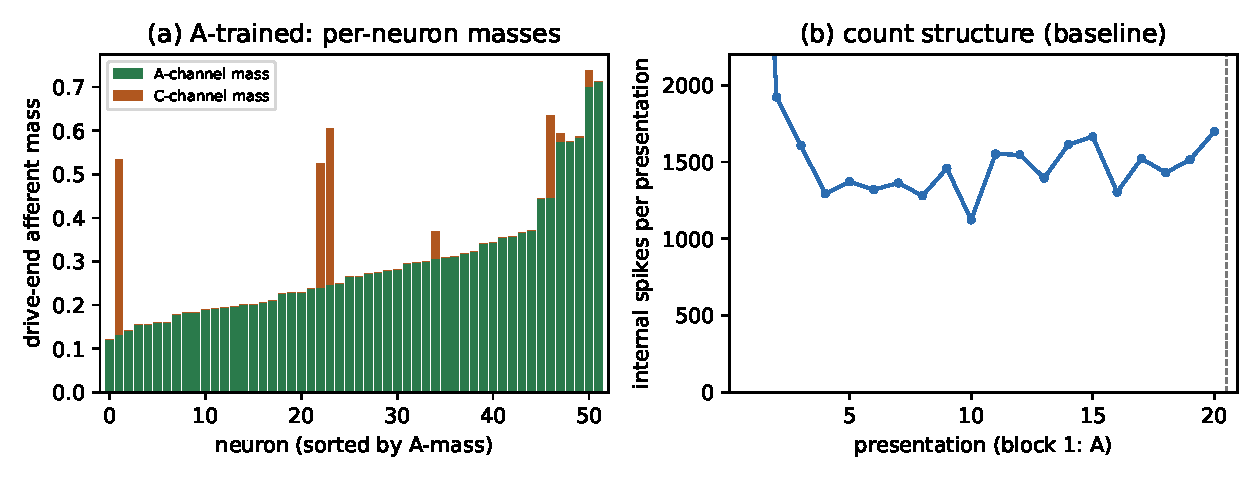
\includegraphics[width=\linewidth]{figures/fig2-organization.pdf}
\caption{\textbf{Emergent sensory organization}. (a) Drive-end
per-neuron afferent mass split (A-channel vs.\ C-channel) for the
A-trained single-pattern run; the population organizes along the
presented channel group (selectivity \(+0.906\), 49/52 neurons)
\cite{synmem}. (b) Per-presentation internal spike counts over the
first (A) block of the baseline blocked run --- the repeatable count
structure that subsequent regimes inherit. Data from preserved runs via
the committed instrument \texttt{rg8eval}.}
\label{fig:organization}
\end{figure}

\section{The Persistent-State Information Bottleneck}\label{sec:bottleneck}
The central diagnostic of Phase I is an information-loss ladder.
Consider what the environment provides and what the persistent variables
of the substrate can possibly retain. Figure~\ref{fig:ladder}
schematizes the cascade; each rung is a compression the substrate
performs automatically, and each was measured where the instruments
allowed.

\paragraph{Rung 1: afferent structure.}
Patterns are channel groups; the persistent synaptic structure develops
selectivity for them (selectivity \(\pm 0.8\)--\(0.9\),
\S\ref{sec:organization}). At this rung, structure exists and survives
silence.

\paragraph{Rung 2: instantaneous spikes.}
At any instant, the internally observed quantity is the spike train.
Spikes carry the full timing information of the stimulus, but they are
activity: the substrate does not store them.

\paragraph{Rung 3: windowed counts.}
The measured representation of a presentation is its 500 ms spike-count
vector. This is the rung at which the organization is assayed
(response separation) and it is stimulus-locked: off-window
(count-free) responses do not separate. The architectural review
measured during-window cross-pattern separation cosines 0.30--0.89 but
off-window 0.999+, and the V2.2-era and E21 records fixed the temporal
carry of the substrate below 50 ms (gap-0 retention only:
\(D_{L{-}NF}=0.0815\)) \cite{overview}.

\paragraph{Rung 4: cumulative counts.}
The substrate has one integrator that accumulates over presentations:
the slow state \(u\) (V2.1), \(u \mathrel{+}= \beta\) per spike with
decay \(\tau_s\). Under drive it saturates to a flux balance (W1 cell:
mean \(u \to \approx 1.32\) by presentation \(\sim\)30). The
integration is over \emph{the organism's own spiking}, which under
drive is stimulus-locked but conflates patterns through the shared
pool (\S\ref{sec:organization}).

\paragraph{Rung 5: intrinsic scalar \(u\).}
What survives into silence is the integrated scalar field. Its
information content is the subject of §\ref{sec:u}: it is a population
rate trace, not a sensory memory.

\subsection{The dilution result across repeated presentations}

The loss that matters for persistent learning is not between rungs 1
and 2 but in what \emph{repeated} presentations do to episode identity
at the persistent rungs. The alternating-regime measurements
\cite{synmem} provide the sharpest quantitative statement: after each
presentation, the state of the synaptic store after an \(A\)
presentation and the state after the adjacent \(C\) presentation
converge --- the cosine of the per-neuron A-mass vector after \(C_k\)
versus after \(A_k\) rises \(0.972 \to 0.990\) over
\(k = 1 \to 40\). Simultaneously the alternating store becomes a
\emph{third configuration}, not a mixture of the trained endpoints
(cosine to the A-only endpoint 0.277, to the C-only endpoint 0.235,
while the endpoints are at 0.119 from each other; the best linear
mixture leaves 96\% of the alternating norm as residual)
\cite{synmem}. In other words: with alternation, episode identity is
diluted to a superposition; with blocking, it is overwritten
(§\ref{sec:interference}); at the persistent rungs the store converges
to quantities that cannot answer ``which episode, most recently.''

The same convergence was first measured in \(u\) (alternating-\(u\)
cosine \(\to 1.0\)) and then reproduced at the synaptic level --- the
records emphasize that the superposition failure is a property of the
shared additive store, not of the particular substrate
\cite{synmem}. Figure~\ref{fig:dilution} plots the two measured faces
of the dilution: the converging adjacent-state cosine (left) and the
within-block response-count decay (right), from the preserved
alternating and blocked runs respectively.

\begin{quote}
\textbf{Demonstrated:} the persistent storage rungs (synaptic weights;
integrated \(u\)) do not retain episode identity under repeated or
alternated exposure; adjacent-episode state similarity rises toward
1 (0.972 \(\to\) 0.990).\\[1pt]
\textbf{Supported:} the loss occurs at the transition from
presentation-local (spikes, counts) to persistent (integrals, weights)
representations; the shared-budget additive store is the mechanism
(later confirmed by the CLLA-era results, §\ref{sec:clla}).\\[1pt]
\textbf{Not established:} any persistent rung that distinguishes recent
episodes --- this is the negative result that motivates the rest of the
paper.
\end{quote}

\begin{figure}[t]
\centering
\resizebox{\textwidth}{!}{%
% Figure 3 — the information-loss ladder (schematic with measured annotations).
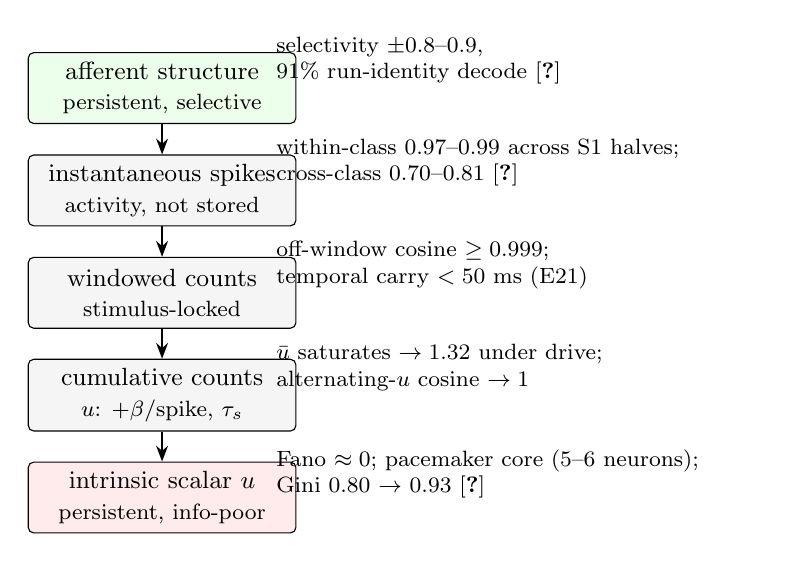
\begin{tikzpicture}[
  rung/.style={draw, rounded corners=2pt, minimum width=3.4cm,
               minimum height=9mm, align=center, font=\small},
  arr/.style={-{Stealth[length=2mm]}, thick}
]
  \node[rung, fill=green!8]  (r1) at (0, 0)   {afferent structure\\\footnotesize persistent, selective};
  \node[rung, fill=gray!8]   (r2) at (0, -1.3) {instantaneous spikes\\\footnotesize activity, not stored};
  \node[rung, fill=gray!8]   (r3) at (0, -2.6) {windowed counts\\\footnotesize stimulus-locked};
  \node[rung, fill=gray!8]   (r4) at (0, -3.9) {cumulative counts\\\footnotesize $u$: +$\beta$/spike, $\tau_s$};
  \node[rung, fill=red!8]    (r5) at (0, -5.2) {intrinsic scalar $u$\\\footnotesize persistent, info-poor};
  \draw[arr] (r1) -- (r2); \draw[arr] (r2) -- (r3);
  \draw[arr] (r3) -- (r4); \draw[arr] (r4) -- (r5);
  % measured annotations
  \node[font=\footnotesize, align=left, text width=6.3cm] (a1) at (4.6, 0.35)
    {selectivity $\pm0.8$--$0.9$,\\91\% run-identity decode \cite{synmem}};
  \node[font=\footnotesize, align=left, text width=6.3cm] (a3) at (4.6, -2.25)
    {off-window cosine $\ge 0.999$;\\temporal carry $< 50$ ms (E21)};
  \node[font=\footnotesize, align=left, text width=6.3cm] (a4) at (4.6, -3.55)
    {$\bar u$ saturates $\to 1.32$ under drive;\\alternating-$u$ cosine $\to 1$};
  \node[font=\footnotesize, align=left, text width=6.3cm] (a5) at (4.6, -4.9)
    {Fano $\approx 0$; pacemaker core (5--6 neurons);\\Gini 0.80 $\to$ 0.93 \cite{infoaudit}};
  \node[font=\footnotesize, align=left, text width=6.3cm] (a2) at (4.6, -0.95)
    {within-class $0.97$--$0.99$ across S1 halves;\\cross-class $0.70$--$0.81$ \cite{e1proto}};
\end{tikzpicture}
}
\caption{\textbf{The persistent-state information bottleneck.}
The substrate's automatic compression cascade: afferent structure
(persistent, selective) \(\to\) instantaneous spikes (activity)
\(\to\) windowed counts (stimulus-locked, not retained) \(\to\)
cumulative counts (the slow integrator \(u\)) \(\to\) intrinsic scalar
\(u\) (persistent but information-poor; §\ref{sec:u}). Each arrow is a
lossy compression performed by the substrate's own dynamics.}
\label{fig:ladder}
\end{figure}

\begin{figure}[t]
\centering
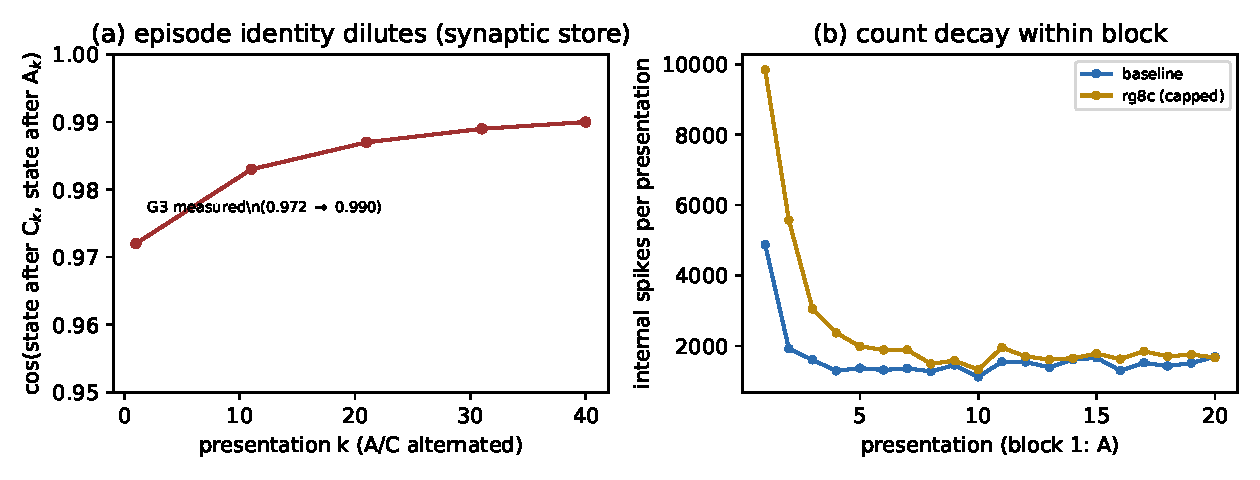
\includegraphics[width=\linewidth]{figures/fig4-dilution.pdf}
\caption{\textbf{Information dilution across repeated presentations.}
Left: convergence of the synaptic store after adjacent \(A\) and \(C\)
presentations under alternation (cosine 0.972 \(\to\) 0.990;
\cite{synmem}). Right: per-presentation internal spike counts decay
within a blocked block (baseline run), the count-level face of the same
dilution. Both measured from preserved artifacts.}
\label{fig:dilution}
\end{figure}

\section{Intrinsic Persistence Is Not Sensory Memory}\label{sec:u}
The slow depolarizing state \(u\) (V2.1) was the designated candidate
for a persistent, intrinsic memory that does not depend on synaptic
structure. Phase I's evidence against that role is unusually complete
because the audits measured what \(u\) actually does during and after
the stimulus, and because one claim was retracted when its runs turned
out not to exist.

\subsection{What \(u\) is, measured}

\(u\) tracks the organism's own spiking through a first-order filter:
per-spike increment \(\beta\), decay \(\tau_s\). Three measured facts
\cite{infoaudit}:

\begin{enumerate}
\item \textbf{It saturates during the stimulus.} Means rise
monotonically with cumulative exposure and plateau at a flux balance
(W1: \(\bar u\to 1.32\) by presentation \(\sim\)30; W2:
\(\bar u\to 0.86\), still rising at drive end). A saturating integrator
cannot encode cumulative episode history beyond its equilibrium.
\item \textbf{Persistence without structure.} After stimulus removal
the population does not relax: the active core self-sustains as
deterministic pacemaking --- 500 spikes/s on the refractory ceiling
(2 ms refractory \(\Rightarrow\) 500 Hz), Fano factors \(\approx 0\),
5--6 active neurons of 52, Gini concentration \(0.80 \to 0.93\) over
silence. The persistent activity is a clock, not a code
\cite{infoaudit}.
\item \textbf{The only tested claim of a discriminative \(u\) is
retracted.} The V2.1 Stage-C validation table claimed temporal-capacity
unchanged at the rule-selected operating point; the referenced runs do
not exist in the repository. The information audit discovered the
phantom reference, retracted the verdict as ungrounded (``unsupported,
not refuted --- unmeasured''), and added an integrity regression that
fails any record citing nonexistent runs \cite{infoaudit}.
\end{enumerate}

\subsection{The historical wedge: \(u\) fails during the stimulus, not only after it}

The standard memory objection to an integrator is that it decays after
stimulus offset. The ANIMA record shows something stronger: in the
regimes where episode identity was tested, the persistent quantities
fail to distinguish episodes \emph{while the stimulus is still
present}. The alternating-store cosine after adjacent \(A\) and \(C\)
presentations converges to 0.99 (\S\ref{sec:bottleneck}) --- the state
after an \(A\) presentation is already near-identical to the state after
the adjacent \(C\), at a measurement taken 2 s apart with exactly one
intervening presentation \cite{synmem}. The V2.2 latch design
(discussed next) was in part motivated by this timing: it attempted to
make a per-neuron bistable bit the carrier, under u-driven SET/RESET
thresholds --- and failed as a carrier (latches decode the curriculum at
chance in all 120 stage-2 runs; \(\eta_{\mathrm{rel}}=1.0\)
self-cancels) \cite{overview}. The E18--E21 temporal-capacity series
bracketed the same wedge from the output side: no antecedent-dependent
divergence over 800 ms; output responses stimulus-locked with zero
endogenous output activity; temporal capacity below 50 ms
\cite{overview}.

\subsection{The drive-gated slow state and the writable-memory review}

The X-series explored the one amendment to \(u\) that its own audit
motivated: gate the per-spike write by the neuron's afferent drive
(\texttt{slow\_state\_beta\_drive}; drive trace
\(x_i = \min(I_{\mathrm{aff}}/v_{\mathrm{th}}, 1)\), fitted with
the frozen membrane scale after the dimensional correction of
\S\ref{sec:repro}; spec and logs
\cite{xspecdrive,xplorlog}). The records measure:
\begin{itemize}
\item X1: a transition band at \(\beta \approx 0.0047\) --- an
intermediate regime with a decaying tail whose effective time constant
(\(\approx\) 8.2 s) differs from \(\tau_u\);
\item X3: a 45-run boundary map in which top-\(u\) at drive end is a
near-perfect predictor of the post-drive regime (\(\rho \approx
0.97\)); drive composition shifts regime, but seed dominates;
\item the architectural review \cite{xplor2}: sensory organization
exists at the afferent layer (42--48 of 52 neurons dominant for a given
pure-drive curriculum; interleaving keeps separable cohorts);
during-stimulus responses separate (cosine 0.30--0.89) while
off-window responses do not (0.999+); the persistent state is a
``seed-lottery'' twice over.
\end{itemize}
The review's primary diagnosis --- \emph{insufficient writable /
competitive memory}; the missing capability is coexisting
independently writeable traces under budget competition --- is the
exact bridge to the synaptic-store chapters: it reframes the negative
as a memory-capability question and names budget competition (M2) as
the suspected mechanism, which the SDE probes and the CLLA era then
isolated \cite{xplor2,overview}.

\begin{quote}
\textbf{Demonstrated:} scalar intrinsic persistence (\(u\)) is
self-sustaining but information-poor (saturated mean, pacemaker core,
Fano \(\approx 0\)); the V2.2 latch carrier failed 120-run tests; the
temporal carry of the substrate is below 50 ms.\\[1pt]
\textbf{Supported:} episode discriminability fails inside the stimulus
window, hence the bottleneck is not post-offset decay but
representation-integration collapse.\\[1pt]
\textbf{Not established / retracted:} the Stage-C capacity claim is
ungrounded and retracted; no A/C contrast in \(u\) was ever executed.
\end{quote}

\section{Synaptic Plasticity as Persistent Structure}\label{sec:synaptic}
If activity rungs cannot persist information, the weights must: they
survive silence by construction (they are only changed by plasticity
events), and the record shows they are the substrate's persistent store.
The plasticity-as-memory audit \cite{synmem} established this with four
independent verdicts.

\paragraph{Persistence (G1, G2).}
Cross-run training (A-only vs.\ C-only, same seed, identical initial
weights) produces distinct persistent configurations: cosine 0.119,
selectivity \(\pm 0.8\)--\(0.9\), 91\% leave-one-pair-out run
identification. Selectivity develops monotonically through S1 and
\emph{continues to develop in silence} (\(+0.903 \to +0.914\), driven by
pruning of residual non-A mass --- 617\(\to\)309 live afferents),
while the matrix itself changes only \(\sim\)1.4\% across 20 s of
silence. Structure persists; activity decays (activity rungs decay
3.5--7\(\times\) in the same window: \(u\)-norm 7.999\(\to\)2.282,
internal spikes 479/s \(\to\) 71/s).

\paragraph{Create/maintain mechanics (G4).}
The causal records (E15--E17, SDE series) attribute organization to a
specific subset of mechanisms: M2 normalization (per-neuron \(t_e\)
budget) is \emph{required} for the separated regime (M2-off destroys
separation; E16), while STDP is not individually necessary for the
afferent-selection trajectory (STDP-off reproduces it near-verbatim,
E16), and M3/M4 topology dynamics are not necessary either (E17).
Maintenance is M2 cadence plus M4 pruning; passive decay
(\(10^{-6}\)/tick) is the dominant single eraser of first-block mass
(SDE-C2: decay-off preserves the first cohort in 6/6 blocked runs;
residual skew \(\approx 0.07\)--\(0.09\) remains). Retrieval is a
dynamics function: the REV1 phase-reversal experiment re-expresses an
early-established configuration with zero plasticity events and
\(\le 3\%\) weight change (E12--E17) --- forward dynamics through
stored weights.

\paragraph{What is not established at this layer (G8).}
Re-expression of a stored configuration by a later input exists at the
association/trace level; \emph{episode-specific} reinstatement under
alternation does not --- the alternating store superposes
(§\ref{sec:interference}) and no later \(A\)-presentation reinstates an
A-configuration distinguishable from the adjacent C-configuration.

\begin{quote}
\textbf{Demonstrated:} synaptic structure is the persistent store;
creation requires budget normalization; retention is bounded by decay
and order; retrieval-by-forward-dynamics exists for trace-level
configurations.\\[1pt]
\textbf{Supported:} the information bottleneck is shared by every
persistent substrate tested (weights and \(u\) show the same
superposition signature), hence the limiting factor is the shared
additive store under a shared budget, not the substrate identity
\cite{synmem}.
\end{quote}

\section{Synaptic Interference: Isolated, Blocked, and Alternating Regimes}\label{sec:interference}
The regime trichotomy --- isolated, blocked, alternating --- is the
organizing experimental fact of the synaptic-structure era. All three
were measured on the same cell (the e24 operating point
\(\beta=0.0046875,\ \tau_s=5000\)), same seeds, with the same
snapshot-based instrument \cite{synmem}; Figure~\ref{fig:regimes} shows
the end-state channel masses.

\paragraph{Isolated.} A single pattern trained to completion yields
clean winner selection: A-mass 0.290 / C-mass 0.026 (A-trained) or the
mirror (0.031 / 0.239, C-trained). The unchallenged group is pruned
away by budget normalization plus M4 selection.

\paragraph{Blocked.} Sequential blocks overwrite: BAC (20 A then 20 C)
ends at A-mass 0.068 / C-mass 0.137 --- the first block's mass is
removed by the second (unmodified substrate; the CLLA-era numbers in
\S\ref{sec:clla} reproduce the same shape under protection). BCA ends
at 0.234 / 0.105. Each blocked run drifts toward its final block's
trained endpoint (cos to its own endpoint 0.52--0.58) but lands between
the endpoints (both blocks leave residual mass).

\paragraph{Alternating.} Both groups remain driven, so neither is
pruned: end-state A-mass 0.239 / C-mass 0.162 --- both retained, no
overwrite. But the retained state is a superposition: it is neither a
mixture of the endpoints (best linear mixture leaves a 96\% residual)
nor a discriminator of the most recent episode (adjacent-state cosine
0.972 \(\to\) 0.990, \S\ref{sec:bottleneck}).

\paragraph{Causal decomposition.} SDE-B (doubling \(t_e\)) showed that
capacity is not the lever: the surplus feeds the dominant trace and
coexistence does not improve. SDE-C2 isolated passive decay as the
dominant eraser of the first block (decay-off preserves first-cohort
mass in 6/6 blocked runs). SDE-D showed the STDP \(a^-/a^+\)
asymmetry is secondary and context-dependent; the leading unresolved
residual mechanism was M2 reallocation (inference at the time, later
supported by the trace-partitioned M2 experiment, V2.3, which rescued
blocked-order collapse-class cells 6/6 by capacity-matched per-bucket
targets \cite{overview}).

\begin{quote}
\textbf{Demonstrated:} isolated \(\to\) winner selection; blocked
\(\to\) recency overwrite; alternating \(\to\) coexistence without
episode discrimination. The trichotomy reproduces at the protected
(CLLA) layer later (\S\ref{sec:clla}) and under all tested amendments
except the M2 partition, which was tested blocked-only.\\[1pt]
\textbf{Supported:} the shared per-neuron additive budget is the
interference medium; passive decay is the dominant eraser; budget
partition is the only measured lever improving blocked coexistence.
\end{quote}

\begin{figure}[t]
\centering
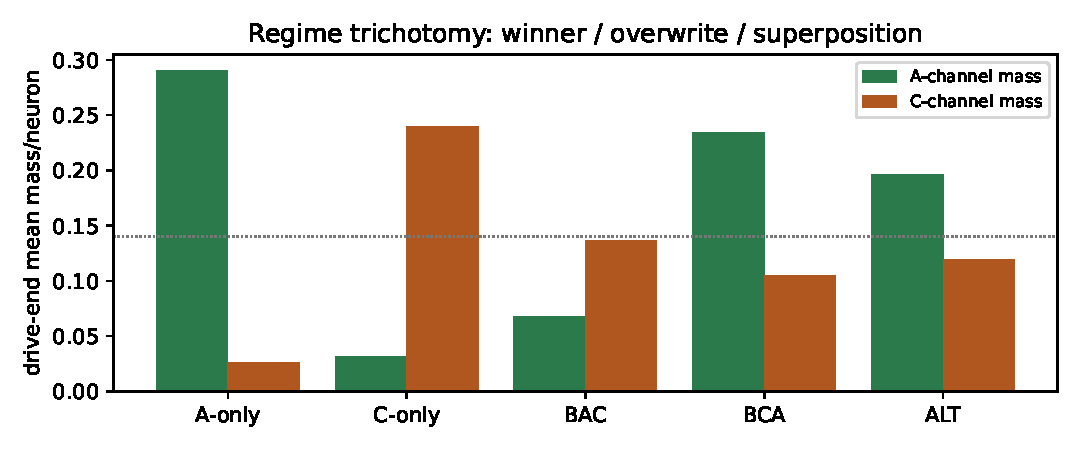
\includegraphics[width=\linewidth]{figures/fig5-regimes.pdf}
\caption{\textbf{Isolated vs.\ blocked vs.\ alternating synaptic
organization} (same cell, same seed; drive-end mean per-neuron channel mass; single-pattern and blocked bars recomputed from preserved
runs by the committed \texttt{papermass} instrument, reproducing the
audit table values at print precision; the alternating bar is the
e24-il run at the same 40-presentation convention (the audit's longer
40+40 alternating run reads 0.239/0.162 --- the same superposition, not
a mixture of the endpoints) \cite{synmem}). Isolated training selects
one channel group; blocked order
overwrites the earlier block; alternation retains both groups but as a
superposition that does not discriminate the most recent episode
\cite{synmem}.}
\label{fig:regimes}
\end{figure}

\section{Consolidation-Locked Allocation (CLLA)}\label{sec:clla}
Consolidation-locked allocation (CLLA) is the Phase I attempt to make
synaptic interference addressable: protect synapses that have reached
permanence, so that later plasticity cannot silently dismantle an
established structure. The sequence of four records is the clearest
example of the program's causal narrowing, and each step is reported
separately because the amendments are protocol changes, not re-runs.

\subsection{The mechanisms}

Three mechanisms, separable in the record:

\begin{itemize}
\item \textbf{Consolidation.} At M3 permanence (candidate weight
\(\ge \theta_{\mathrm{perm}}=0.05\)), a synapse may be flagged
\emph{consolidated} (\texttt{assembly\_protect} on): it becomes exempt
from M2 rescaling, M4 silence-pruning, and passive decay.
\item \textbf{Bounded protected mass.} Consolidated LTP is clipped so
that per-neuron protected mass \(P_i = \sum_{\text{consolidated}} w\)
satisfies \(P_i \le p_{\max} t_e = 0.60\) at every tick
(the bounded-protection amendment; \cite{bbounded}).
\item \textbf{Residual allocation gate (later).} Candidate
accumulation gated by the protected-current fraction
\(R_i = I_{p,i}/(I_{p,i} + I_{w,i})\), so unconsolidated (``unexplained'')
drive keeps allocation priority; \S\ref{sec:allocation}.
\end{itemize}

\subsection{The four-record sequence}

\textbf{1. Unbounded protection --- runaway.} With consolidation but no
growth bound, protected synapses are exempt from every brake (M2,
decay) while STDP still applies: within-pattern LTP runs unimpeded, P
reaches \(\approx 7.9\)/neuron against the 0.60 cap (cap violations
2{,}284--3{,}408 per surviving run; max \(P/(0.75t_e) = 13.3\)), and 6
of 12 runs abort on the runaway detector (50 Hz/5 s). Verdict:
bundle NOT SUPPORTED, failure mode F3/F4 --- protection without a
homeostatic bound is unstable \cite{cllarecord}.

\textbf{2. Bounded protection --- viability.} The amendment clips
consolidated LTP at the remaining headroom. All 12 runs complete;
protected mass pins at 0.6000 (f32-exact) everywhere; working budget
stays strictly positive (\(t_e - P \ge 0.2\)); rates settle to
3.5--6.5 Hz; the previously-aborting cells complete. Verdict:
dynamically viable \cite{bbounded}.

\textbf{3. Capability --- coexistence split.} The frozen falsifier F1
requires drive-end channel mass \(\ge 0.5\times\) per-seed
single-pattern reference in all arms. Alternating (il) passes 3/3
(protected-ratio A/(A+C) 0.53--0.59); blocked (bac/bca) fails 6/6:
the later block captures the shared working budget and the protected
slots (bac ends C-poor: C 0.101/0.057/0.037; bca ends A-poor:
A 0.116/0.056/0.055). F3 (cap), F3b (exhaustion), F4 (stability),
F5 (no hidden context), F7 (protected-mass retention, ratios
0.80--1.00) pass 12/12. F2/F6 are unmeasurable under the frozen windows
(empty by curriculum construction --- a recorded protocol defect,
\S\ref{sec:method}); the closest-available-window diagnostics are
consistent with late separation (cross 0.15--0.40, within 0.85--0.89
in all three il runs). Verdict: bundle NOT SUPPORTED, with the failure
localized to \emph{allocation} --- blocked-order recency capture --- not
protection, stability, or retention \cite{capability}.

\textbf{4. Interpretation split.} The records draw the distinction that
organizes the rest of Phase I:
\begin{quote}
\textbf{Protection} (bounded) is established: retained, capped,
stable.\\
\textbf{Coexistence} is order-dependent: demonstrated under
alternation, absent under blocked order.\\
\textbf{Allocation} --- who gets the budget and the protected slots when
patterns arrive sequentially --- is the unresolved capability that the
remaining experiments attack.
\end{quote}

Figure~\ref{fig:protection} shows the bounded-protection witness
trajectory: protected mass fills to the cap and pins there while the
working pool shrinks, without instability.

\begin{figure}[t]
\centering
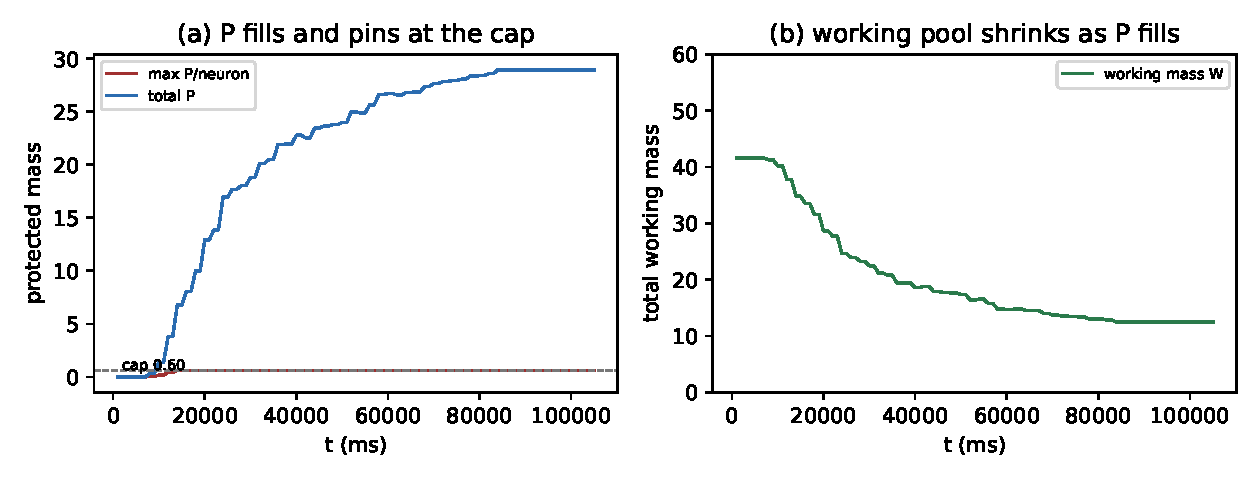
\includegraphics[width=\linewidth]{figures/fig6-protection.pdf}
\caption{\textbf{CLLA bounded protection: stability at the cap.}
Per-snapshot (1 s) trajectories of the previously-aborting
s424242-il cell under the bounded amendment: per-neuron protected mass
\(P\) rises to and pins at the 0.60 cap; total protected mass grows as
more neurons fill; the working pool \(W\) shrinks to the residual
budget as protection fills; zero failures (all 12 runs complete)
\cite{bbounded}.}
\label{fig:protection}
\end{figure}

\section{Allocation Experiments}\label{sec:allocation}
With stability established, the frozen question became allocation:
\emph{can a local mechanism prevent first-arrival starvation of a later
distinct configuration?} Each registered experiment tightened the
answer and moved the identified bottleneck one step downstream. All
five share the identical identity gate (flag-off byte-identity
\texttt{9647ea8a0ca4dbd2}), the identical 12-run matrix (bac/bca/il/d
\(\times\) three seeds), and the identical primary endpoint:
second-block protected mass \(\ge 0.5 \times\) first-block protected
mass.

\subsection{Residual allocation gate (rule)}

The gate (protocol \cite{cllaprot} extension, record \cite{rule})
multiplies candidate accumulation by \(g_i = \max(0,1-R_i)\) with
headroom > 0, where \(R_i = I_{p,i}/(I_{p,i}+I_{w,i})\) is the
protected-share of the neuron's delivered input current. The
implementation behaves exactly as specified --- the gate sat at
\(g = 1.0\) through the entire second block (\(R\)-median 0.000),
headroom was reserved (0.249--0.294 vs.\ 0.155--0.161 in the no-rule
runs), and first-block permanence decelerated (170 events, 8.5/pres,
vs.\ 364, 18.2/pres) --- yet the primary endpoint failed 6/6 (ratios
0.008--0.192 vs.\ the 0.5 bar). The trajectory instrument located the
failure \emph{upstream of the rule}: the second-block working substrate
is destroyed during the first block (live unconsolidated C-channel
afferents \(197 \to 77\) under M2 normalization of the shrinking
working budget and M4 pruning), so at second-block onset
\(g=1\) with almost nothing to accumulate. Verdict: the gate is not the
bottleneck; substrate availability is \cite{rule}. Alternating
coexistence preserved (F1-il 3/3).

\subsection{Dormant-candidate reserve}

The reserve (record \cite{reserve}) lets ever-coactive candidates
survive dormancy at a floor instead of dying, protecting pre-associations
across inactive periods. The mechanism works measurably --- 90--255
reserved candidates per run survive --- but at second-block onset in the
blocked arms the reserved C-cohort (channels 8--15) is exactly
\emph{zero} (mean over the A block: reserved A-cohort 123.7, C-cohort
0.0); the block-2 permanence count is 38 vs.\ 35 without the reserve.
The record classifies the outcome as \emph{neither} preservation
failure \emph{nor} flux failure: a trigger keyed on ``ever-coactive''
is satisfiable only by the pattern that has already been active. The
reserve is vacuous for a genuinely first-seen pattern by the semantics
of its own trigger \cite{reserve}.

\subsection{First-exposure allocation}

The next amendment biases candidate redraw/eviction toward channels
that fired in the current window, so a currently active novel input can
bind candidate slots before churn eliminates its substrate (record
\cite{fe}). Primary endpoint still failed 6/6 (ratios 0.072--0.216),
but the causal path became exact: first C permanence at \(t = 47{,}400\)
--- 2.4 s after block onset, 10\(\times\) faster than baseline;
permanence events 41 vs.\ 35 (allocator-only) and 38 (reserve);
block-1 allocation \emph{increased} (248 vs.\ 170 events --- the
mechanism strengthens whatever is currently active). The binding supply
was capped by two interacting facts: only \(\approx 0.71\) visible
channels/neuron survived at onset (visibility cap), and the
redraw-bias branch was structurally inert (\texttt{connected()}
excludes exactly the visible channels it would have preferred). The
implementation audit (\cite{feimpl}) identified the latter as a spec
vacuity --- the bias could never fire --- and the next amendment
corrected the source.

\subsection{Source-selection correction}

The corrected source reads the module's per-window firing record
instead of afferent-derived channel sets, making all firing channels
observable regardless of synapse survival (record \cite{fec}). Supply
tripled (41 \(\to\) 61 C-cohort permanence events); first permanence at
2.5 s; primary endpoint still failed 6/6 (ratios 0.046--0.193).
The classification that survived into the paper's central question:
flux improved but remained asymmetric (3.05/pres C vs.\ 13.2/pres A),
and the measured residual bottleneck was \emph{post-permanence weight
growth + working-afferent churn} --- newly protected second-block
synapses consolidate at \(w\approx 0.02\) and grow little (mean 0.054
vs.\ the first block's 0.096) because the working C afferents that
would drive their LTP keep being destroyed (29 \(\to\) 11 across the
second block itself) by M2's working-mass squeeze. The record
registered the two candidate amendments it did not run (e1:
consolidation-time protection of a working-afferent fraction; e2:
protected-path LTP growth) \cite{fec}. Figure~\ref{fig:decomp} plots
the final state of this decomposition.

\subsection{What the sequence ruled out}

\begin{itemize}
\item Allocation gating: \textbf{ruled out as the limiter} --- the gate
did nothing wrong and changed nothing.
\item Dormant preservation: \textbf{ruled out} --- preservation works,
but has nothing preservable before first contact.
\item First-exposure visibility: \textbf{fixed then ruled out} --- the
source correction removed the vacuity; supply tripled.
\item Flux (candidate accumulation rate): \textbf{supported as
secondary} --- asymmetric (3.05 vs.\ 13.2/pres) but not the binding
constraint.
\item Working-substrate churn against the \emph{new} protected
structure: \textbf{the measured residual} --- leads directly to the
recruitment question (\S\ref{sec:recruitment}).
\end{itemize}

\section{The Novel-Pattern Recruitment Bottleneck}\label{sec:recruitment}
The allocation sequence ended with a measured paradox: the corrected
allocator could deliver candidate substrate (permanence supply tripled),
and yet the second block's protected structure stayed at \(\approx
1/10\) of the first block's mass. The resolution required decomposing
what a newly consolidated synapse needs \emph{after} permanence: LTP
support from co-firing postsynaptic activity. Two read-only audits
\cite{wgrowth,drive}, both over the committed source-correction runs
(registration-era baselines of \S\ref{sec:rg}), localized the failure
to the very first link of the second block.

\subsection{Event-level decomposition (weight-growth audit)}

For the 61 C-cohort permanence events of the second block in the
baseline blocked run, the per-synapse decomposition is complete
\cite{wgrowth}:

\begin{itemize}
\item starting weight at permanence: \(w_{\mathrm{c,perm}}=0.02\)
(snapshot-verified);
\item pre-spikes: abundant --- C channels fire 56--87 spikes per
500 ms presentation; the input side is not starved;
\item post-spikes: the decisive deficit --- the last A presentation
fires 1{,}697 internal spikes; the first C presentation fires 101;
C presentations sustain 101--222 (a 17\(\times\) collapse at the
block switch; A-block presentations run 1{,}300--1{,}700);
\item applied LTP: the STDP balance on the C cohort over the C block is
\emph{net negative} (\(-21.63\) over 1{,}961 coalesced events): with
post activity so sparse, the dominant pre/post pairing is LTD;
\item per-synapse growth is intact whenever posts exist (measured
factors of 2.5--3.8\(\times\), e.g.\ \(0.02 \to 0.185\));
\item M2 is not suppressing: the working target stays
0.360 \(\to\) 0.303 across the block (per-neuron \(P\)
0.44 \(\to\) 0.50, cap 0.60);
\item M4 is quiet in the second block: 23 C-afferent prunes vs.\ 161 in
the first block;
\item causal order: the post-activity collapse (pres-21) precedes every
C permanence (first at \(t=47{,}500\), 2.5 s after onset) and all C
weight growth.
\end{itemize}

Verdict: \textbf{event-limited (A)} --- second-block C fails at the
level of relevant postsynaptic LTP opportunities; the growth machinery
works where posts exist.

\subsection{Drive decomposition and the IL control (drive audit)}

Why do C presentations produce a hundred spikes instead of a thousand?
The drive audit \cite{drive} decomposed the first-exposure currents
(per-neuron means, snapshot + spike telemetry):

\begin{center}
\footnotesize
\begin{tabular}{lcc}
\toprule
quantity (first exposure, per neuron) & first-A (block 1, pres 1) & first-C (block 2, pres 21) \\
\midrule
afferent current \(I_{\mathrm{aff}}\) & 11.98 & 1.57 \\
recurrent current \(I_{\mathrm{rec}}\) & 6.90 & 0.05 \\
inhibitory current \(I_{\mathrm{inh}}\) & \(-2.19\) & \(-0.81\) \\
posts/n & 0.98 & 0.12 \\
\bottomrule
\end{tabular}
\end{center}

The first-C presentation delivers \(\approx 7.7\times\) less afferent
current than the first-A presentation did, all of it working
(unconsolidated): block-1 churn (M2 working-budget squeeze + M4
pruning, dominated by passive decay per SDE-C2) reduced the live C
working afferents from \(\approx 197\) to \(\approx 29\) before C was
ever presented. With 1.6 drive/neuron and no recurrent support, the
population sits below threshold; no posts; no recurrent bootstrap; the
LTD-dominant STDP balance; protected structure starves. M6 inhibition is
excluded as the cause: it is 2.7\(\times\) \emph{lower} at first C than
at first A (it follows activity, it does not create the deficit).

The control that converts this from correlation to causation is the
interleaved regime. In the committed alternating runs, C is present
from presentation 1, so its substrate is never churned; first-C
afferent current is 11.13/neuron, recurrent 7.05, posts 1.00 ---
numerically identical to A's first contact --- and C permanence (98)
matches A (95) \cite{drive}. The blocked-vs-alternating comparison
isolates \emph{prior representation / substrate competition} as the
variable: the C stimulus itself is intrinsically fine.

\begin{quote}
\textbf{Demonstrated:} first-exposure drive for a late pattern is
\(\approx 8\times\) below first-block levels because its working
substrate was destroyed before exposure (prunes +18--31\%; passive
decay family per SDE-C2); posts collapse 17\(\times\); the mechanism is
event-limited, not LTP-, M2-, or M4-limited.\\[1pt]
\textbf{Supported:} the deficit is curriculum-inherent (blocked-order
churn); the alternating regime recruits symmetrically without any
added mechanism.
\end{quote}

\begin{figure}[t]
\centering
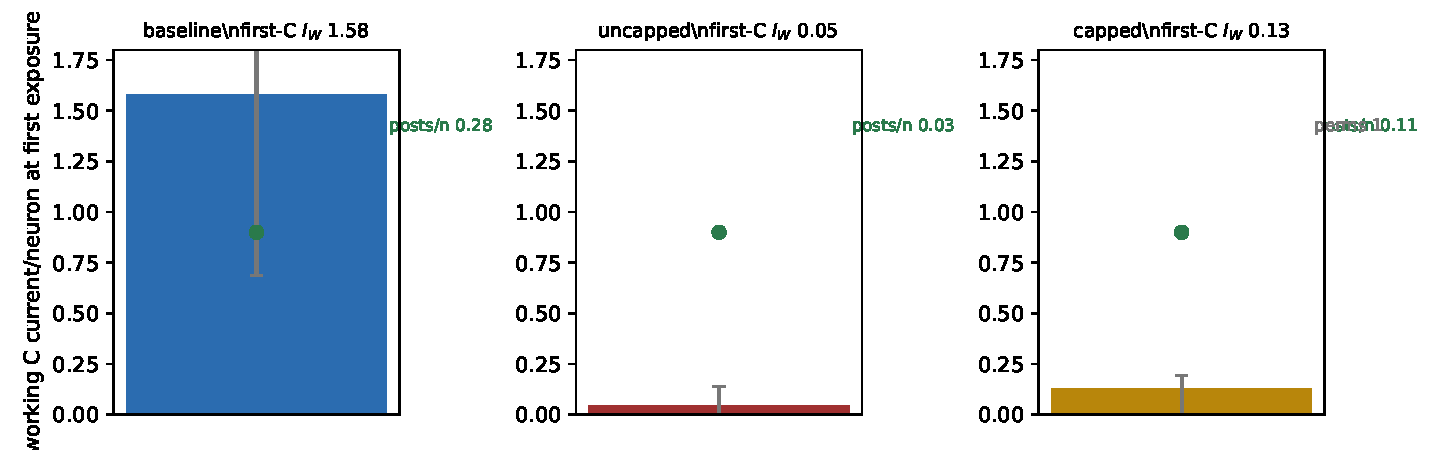
\includegraphics[width=\linewidth]{figures/fig7-decomp.pdf}
\caption{\textbf{Allocation/recruitment failure decomposition} at first
exposure of the late pattern (blocked runs, three seeds; bars show
mean over seeds, ticks the range). Left: working afferent current
surviving to first exposure (baseline 1.565/neuron) collapses under the
uncapped gain and is only partially rescued by the cap. Center: first-
exposure posts/n. Right: second-block permanence events (bar 150).
All panels from preserved runs via the committed \texttt{rg8eval}
instrument \cite{rg8,rg8c}.}
\label{fig:decomp}
\end{figure}

\section{The Fixed-\(k_g\) Recruitment-Gain Experiment}\label{sec:rg}
The recruitment audits localized the bottleneck; the fixed-mechanism
experiment tested the smallest hypothesized amendment: a local,
novelty-dependent recruitment gain that transiently raises a neuron's
recruitability when its input is unexplained and its post activity is
sparse. The design review \cite{designreview} derived the form from
existing local quantities only --- the allocation rule's unexplained
fraction \(1-R\) and the neuron's own working input current \(I_W\) ---
and concluded that a single new dimensionless magnitude \(k_g\) was
unavoidable (every existing constant is \(\le 1\times\); the required
bootstrap is \(\ge 6\)--\(10\times\) under the measured drive\(\to\)
posts map, whose middle band [4.2, 19] current units is unmeasured by
any committed presentation). Per the pre-registration mandate the
parameter was not fitted: the user froze the first mechanism test at
the lowest defensible value,

\begin{equation}
  i_{\mathrm{boost},i}(t) = k_g \cdot \max(0,\, 1 - R_i(t)) \cdot I_{W,i}(t),
  \qquad k_g = 8.0,
  \label{eq:rg}
\end{equation}

with everything else byte-identical to the committed configuration,
including the identity gate and the frozen endpoint bars
\cite{designreview}. The experiment was executed in two registered
arms.

\subsection{Registration A: uncapped (k\_g = 8.0)}

Nine gain arms (bac/bca/il \(\times\) three seeds) against the nine
committed baselines, all flag-off byte-identical \cite{rg8}.
Endpoints: 4a zero runaway trips (PASS, failures \([]\) in all arms);
4b block-1 first-exposure burst band (FAIL --- pres 1--5 mean
185.9--201.0 Hz vs.\ the [100, 200] Hz bar, with pres-1 at 391--449 Hz
vs.\ 57--94 baseline); 4c first-pattern posts at presentation 20
preserved (PASS, ratio 1.00--1.04); 4d protected cap (PASS, pinned at
0.6000 as in baseline); and the three primary recruitment endpoints
(all FAIL): first-novel posts/n \(\ge 0.5\) (measured 0.00--0.19),
novel permanence \(\ge 150\) (0--22), protected novel end-mass
\(\ge 0.09\) (0.000--0.058).

The mechanism of failure was measured, not inferred: the full-gate
boost on the \emph{first block's own} first exposures
(\(I_W \approx 12\), \(R=0\) \(\Rightarrow\) boost \(\approx 96\),
drive \(\approx 108\) vs.\ the normal 38) drove pres-1 bursts to
391--449 Hz; the hyperactive block then \emph{accelerated} the churn
that destroys the late pattern's substrate (C-cohort prunes in block 1:
195--215 vs.\ 164--187), so at first C exposure the surviving working
current was 0.000--0.14/neuron vs.\ 1.565 baseline --- and the boost is
input-proportional: \(I_W = 0 \Rightarrow\) boost \(= 0\) by
\eqref{eq:rg} itself. The mechanism never engaged at its target moment.
Per the frozen interpretation rule, a 4b failure classifies as a
\emph{recruitment-gain operating-point failure first}; the weak-pattern
recruitment hypothesis was not falsified by registration A
\cite{rg8}.

\subsection{Registration B: threshold-completion cap}

The separately registered amendment \cite{rg8c} clamps the boost at the
current needed to reach threshold in one step,

\begin{equation}
  i_{\mathrm{boost},i}(t) = \min\!\Big(
    k_g \cdot \max(0,1-R_i(t)) \cdot I_{W,i}(t),\;
    \max(0,\,(v_{\mathrm{th}} - v_i(t))\,\tau_m/dt)
  \Big),
\end{equation}

parameter-free (existing \(v_{\mathrm{th}}=1\), \(\tau_m = 20\),
\(dt=1\)); the clamp was implemented per-\emph{neuron} after a
per-synapse first pass was caught in review, with a discriminating unit
test (two afferents, summed raw boost 41.6 \(>\) cap 20 \(\Rightarrow\)
one clamped boost). Identity gate and suites passed; all nine arms
completed, zero failures.

Results against the same bars \cite{rg8c}: 4a PASS; 4b aggregate
5-presentation means 175.6--189.1 Hz inside the band --- but pres-1
remained 378--440 Hz, and under the strict per-presentation reading 4b
is still outside the band in every arm; the cap moved pres-1 only
391 \(\to\) 378 Hz. The mechanism is now understood: the per-tick cap
tops a below-threshold neuron to threshold on every tick while input is
ongoing, sustaining \(\approx 1\) spike/tick (refractory-limited)
regardless of boost magnitude --- the overshoot is
rate-sustained, not magnitude-sustained. The primary endpoints still
failed everywhere (first-novel posts 0.00--0.19; novel permanence
5--15; protected novel end-mass 0.000--0.092, reaching 0.09 in exactly
one arm with only 5 protected synapses); IL preservation stayed partial
(C posts 1.08--1.21\(\times\), permanence 97/74/105 vs.\ the \(\pm20\%\)
of 98 band); gap activity remained elevated (2.3--27.0 vs.\
0.45--5.94 Hz baseline).

\subsection{Why the experiment was closed}

Per the pre-registered outcome rules, each arm was closed at its
failure: no reparameterization, no bracketing, no post-hoc threshold
change, no E-number. The honest verdict language of the records is
preserved here:

\begin{quote}
Registration A: \textbf{operating-point failure} --- 4b fails; the
weak-pattern recruitment hypothesis is \emph{not falsified} (the
mechanism never fired at first exposure because its own block-1 side
effect destroyed the substrate it amplifies).\\[2pt]
Registration B: the cap repairs the aggregate operating point but not
the first-exposure rate; the primary endpoints fail everywhere. The
measured reason is structural: churn precedes exposure (even capped,
block-1 prunes of the late cohort run 193--221 vs.\ 157--187
baseline), and the boost is input-proportional, so a membrane-side gain
has almost nothing to amplify at first contact (surviving working
current 0.00--0.19/neuron vs.\ 1.565). Under the registration B
outcome rule (4b pass + primary fail \(\Rightarrow\) falsified at this
substrate), the records state the hypothesis as \emph{falsified at this
substrate under the corrected operating point}, while noting that
neither registration achieved a clean block-1 operating point, so the
falsification claim is bounded by the residual operating distortion
\cite{rg8c}.
\end{quote}

Both registrations were closed per protocol; the threshold-completion
cap is recorded as the designated, tested alternative; no further
parameter was selected from the results.

\section{Phase I Synthesis}\label{sec:synthesis}
Phase I's net result is a capability map with a single open frontier.
Table~\ref{tab:capability} states the capability, the status, and the
record that establishes or withholds it. Each entry was verified
against the cited record before inclusion.

\begin{table}[t]
\centering
\caption{\textbf{Phase I capability matrix}. Statuses: \emph{established}
(measured, reproduced), \emph{supported} (consistent evidence,
non-decisive protocol slots), \emph{insufficient} (measured, failed its
role), \emph{demonstrated under condition} (order-dependent),
\emph{not established}.}
\label{tab:capability}
\footnotesize
\begin{tabular}{p{3.4cm}p{5.4cm}p{6.4cm}}
\toprule
Capability & Status & Record \\
\midrule
Sensory organization (afferent) & established & G1/G2 \cite{synmem} \\
Transient representation (per-presentation counts) & established & E1 \cite{e1proto} \\
Synaptic reorganization & established & G1/G4 \cite{synmem} \\
Scalar intrinsic memory (\(u\)) & insufficient & info audit \cite{infoaudit} \\
Temporal (sub-50 ms) episode carry & not established (measured \(<\) 50 ms) & E21 \cite{overview} \\
Protected synaptic structure & established & bounded CLLA \cite{bbounded} \\
Alternating coexistence & demonstrated & CLLA F1-il \cite{capability} \\
Blocked-order coexistence & not established (overwrites) & F1-blocked, G3 \cite{capability,synmem} \\
Sequential allocation & unresolved & rule/reserve/fe/fec \cite{rule,reserve,fe,fec} \\
First-exposure substrate survival & not established & fec residual (e) \cite{fec} \\
Novel-pattern recruitment & unresolved & rg8/rg8c \cite{rg8,rg8c} \\
General retrieval (episode-specific) & not established & G8 \cite{synmem} \\
Homeostatic structural growth & not viable under the tested substrate (regressions) & E4 series \cite{e4proto} \\
Closed-loop memory behavior & not established & E19--E23 \cite{overview} \\
\bottomrule
\end{tabular}
\end{table}


The causal narrowing itself is the paper's thesis, and
Figure~\ref{fig:capmap} presents it as a chain of measured limits:

\begin{enumerate}
\item the substrate organizes (afferent selectivity \(\pm 0.9\),
  91\% run-identity decode);
\item transient representations exist (stimulus-locked counts;
  separation resisted E3/E3b dynamics interventions);
\item long-horizon accumulation destroys episode identity (adjacent-
  state cosine \(\to 0.99\); LOPO fails under alternation);
\item scalar intrinsic persistence is information-poor (saturated
  integrator, pacemaker core, Fano \(\approx 0\); latch carrier fails);
\item synaptic structure becomes the persistent substrate
  (structure persists, activity decays; decay is the dominant eraser);
\item synaptic interference appears as order dependence (isolated
  selects, blocked overwrites, alternating superposes);
\item protection restores stability (bounded CLLA: cap pinned, zero
  failures) but not allocation;
\item allocation becomes limiting (gate, reserve, first-exposure:
  each moved the identified site downstream);
\item first-exposure allocation becomes limiting (source correction
  tripled supply; post-permanence growth starved);
\item novel-pattern recruitment becomes limiting (17\(\times\) post
  collapse; 8\(\times\) drive deficit at first contact; IL control
  symmetric);
\item Phase I closes with that capability unresolved (both gain
  registrations closed by pre-registered rules; hypothesis bounded,
  not destroyed).
\end{enumerate}

Each link is a registered experiment or read-only audit with its run
record; no link is asserted from correlation alone (the IL control and
the pre-exposure-vs.-during-exposure ordering supply the causal
anchors).

\begin{figure}[t]
\centering
\resizebox{\textwidth}{!}{%
% Figure 8 — Phase I capability map (colored grid).
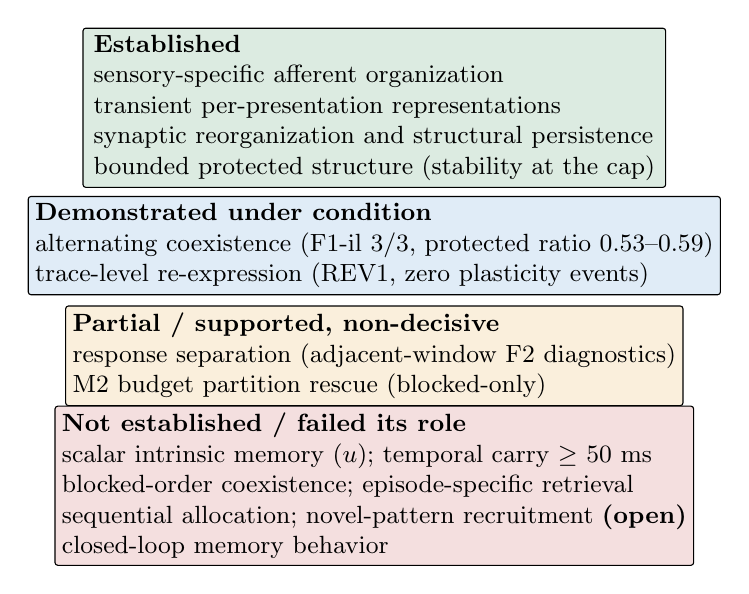
\begin{tikzpicture}[
  cell/.style={draw, rounded corners=1pt, minimum width=7.4cm, font=\small, align=left, inner sep=2.5pt}
]
  \node[cell, fill=cEst!15] at (0, 0)    {\textbf{Established}\\
    sensory-specific afferent organization \\
    transient per-presentation representations \\
    synaptic reorganization and structural persistence \\
    bounded protected structure (stability at the cap)};
  \node[cell, fill=cDem!15] at (0, -1.75) {\textbf{Demonstrated under condition}\\
    alternating coexistence (F1-il 3/3, protected ratio 0.53--0.59) \\
    trace-level re-expression (REV1, zero plasticity events)};
  \node[cell, fill=cPar!15] at (0, -3.15) {\textbf{Partial / supported, non-decisive}\\
    response separation (adjacent-window F2 diagnostics) \\
    M2 budget partition rescue (blocked-only)};
  \node[cell, fill=cNo!15] at (0, -4.8)   {\textbf{Not established / failed its role}\\
    scalar intrinsic memory ($u$); temporal carry $\ge$ 50 ms \\
    blocked-order coexistence; episode-specific retrieval \\
    sequential allocation; novel-pattern recruitment \textbf{(open)} \\
    closed-loop memory behavior};
\end{tikzpicture}
}
\caption{\textbf{Phase I capability map.} Green: established.
Blue: demonstrated under the alternating condition. Amber: partial /
supported-but-non-decisive. Red: not established / failed its assigned
role. The chain reads as the causal narrowing of the persistent-learning
failure described in the text; the final cell (novel-pattern
recruitment) is the open frontier.}
\label{fig:capmap}
\end{figure}

\section{Limitations}\label{sec:limitations}
The record is deliberately narrow, and the following limitations bound
every claim in this paper.

\paragraph{Scale and stimulus regime.}
All CLLA-era results use one organism size (52 internal/output
neurons), three seeds, 8-channel synthetic Poisson patterns at 20 Hz,
and one operating cell (\(\beta = 0.0046875\), \(\tau_s = 5000\) ms).
Scale studies (E7/E8) exist but were not part of the allocation and
recruitment sequence; no claim about larger substrates is made.

\paragraph{No closed loop.}
Nothing in Phase I closes a behavior loop. E19--E23 showed output
activity is stimulus-locked and (in E23) that consequence shaping
exists but inverts; closed-loop memory behavior is listed as not
established.

\paragraph{Protocol defects bound several verdicts.}
The CLLA capability F2/F6 verdicts are formally unmeasured (empty
frozen windows; adjacent-window diagnostics only). The V2.1 Stage-C
claim is retracted. The fe-era afferent-derived source was vacuous and
was corrected; the recruitment design review's drive\(\to\)posts map
has an unmeasured middle band, so bootstrap magnitudes were bracketed,
not calibrated. Each is reported where it matters.

\paragraph{Operating-point confounds.}
First-exposure burst overshoots (baseline D arm peaks 138.8 Hz;
gain registration pres-1 378--449 Hz) sit near the runaway threshold.
The gain experiments were closed with the operating point not fully
clean under the strict 4b reading, which bounds the strength of the
falsification claim recorded for registration B.

\paragraph{Theoretical claims are minimal.}
The paper does not claim biological fidelity, optimality, or any
statement about what real nervous systems must do; the substrate is
four LIF populations with textbook plasticity, studied as an
experimental system. Interpretive claims (``the shared additive budget
is the interference medium'') are labeled supported-versus-hypothesis
in the text.

\paragraph{What is not claimed about failure.}
``Not supported'' and ``not established'' are never converted into
``impossible.'' In particular: the recruitment-gain hypothesis is
bounded by two registrations at one magnitude; other operating points,
other gain forms, and substrate-preserving mechanisms are untested.
Alternating coexistence being demonstrated does not establish general
memory capability; it establishes coexistence under alternation.

\section{Discussion}\label{sec:discussion}
\subsection{Representation}

Phase I demonstrates that a minimally specified spiking substrate
develops sensory-specific organization (afferent selectivity
\(\pm 0.8\)--\(0.9\); 91\% run-identity decode of per-neuron afferent
vectors; repeatable per-presentation count vectors). It equally
demonstrates that the transient representation is weak where it
matters: cross-pattern response separation stalled near 0.67--0.74
against a 0.60 bar, and the two dynamics interventions (adaptation,
lateral inhibition) moved it in the wrong direction
\cite{e1proto,e3bproto}. The binding problem of this organism is
representational: 24 afferents drive one 40-neuron recurrent pool
through random sparse wiring, so every readout mixes patterns. Nothing
in the record suggests this is fixable by further rate dynamics; the
only lever that has ever moved coexistence is budget partition (V2.3,
blocked-only) \cite{overview,synmem}.

\subsection{Persistence}

Persistence has two measured faces. Structural persistence is real and
bounded by mechanics: weights survive silence (matrix drift \(\sim
1.4\%\)/20 s), decay is the dominant eraser (SDE-C2), and bounded
protection stops the runaway that unbounded protection caused
\cite{bbounded,cllarecord}. Activity persistence is information-poor:
the V2.1 slow state self-sustains but saturates, and its endogenous
form is deterministic pacemaking \cite{infoaudit}. The paper's
strongest persistence claim is negative and precisely delimited: no
persistent substrate measured in Phase I retains episode identity
through repeated or alternated exposure --- including, in the testable
case, during the stimulus itself.

\subsection{Interference}

Interference is order-dependent and budget-mediated. Isolated
training selects; blocked training overwrites; alternation superposes
into a third configuration. The causal probes attribute the erasure to
passive decay acting through M2's shrinking working budget, with M4 as
the executing pruner; STDP's \(a^-/a^+\) asymmetry is secondary
(SDE-D). Protection fixes stability, not interference: even with
bounded protected structure, blocked order captures the budget for the
latest block \cite{capability}. Interference is therefore best
described as an \emph{allocation} phenomenon --- competition for a
shared local budget --- rather than a plasticity-sign phenomeno.

\subsection{Allocation}

The allocation sequence is the paper's procedural core: five
registered experiments, each gated byte-identical, each moving the
identified bottleneck one step downstream (gate \(\to\) trigger
semantics \(\to\) visibility \(\to\) source \(\to\) post-permanence
growth). The final measured residual is that the working substrate of a
not-yet-presented pattern is dismantled before its first exposure, and
that even a corrected allocator cannot grow the protected structure
once substrate is gone. This is the point where Phase I's causal
narrowing arrives at the architectural frontier: allocation works when
the pattern is active, and fails for patterns that have never been
active --- which is exactly the class that sequential memory requires.

\subsection{Recruitment}

The recruitment deficit is the frontier's content: a genuinely new
late-arriving pattern cannot recruit postsynaptic activity because its
afferent substrate was churned away, and no membrane-side,
input-proportional gain can amplify a substrate that is not there. The
IL control proves the stimulus is not at fault. Two registered
mechanism tests bounded the hypothesis without resolving it; the
threshold-completion cap fixed the aggregate operating point but could
not repair first-exposure rate or substrate survival. The discussion
stops here by intent: Phase I's evidence supports a direction
(architectures for multiple independently retrievable persistent
representations under sequential experience), not a design.

\section{Conclusion}\label{sec:conclusion}
ANIMA Phase I investigated emergent organization and the architectural
limits of persistent learning in a minimally specified spiking nervous
system. Under frozen protocols, byte-identical identity gates, and
preserved negative results, the record demonstrates that:

\begin{itemize}
\item sensory-specific synaptic organization emerges from local
plasticity without supervision;
\item transient spike-count representations exist but separate poorly
across patterns;
\item every persistent substrate tested --- the slow intrinsic state
and the synaptic weight structure alike --- fails to retain episode
identity through repeated or alternated exposure, in the testable case
already during the stimulus;
\item bounded consolidation produces stable protected structure and
preserves alternating coexistence, but blocked-order allocation
remains recency-dominated;
\item the allocation sequence localized the residual failure to the
working-substrate churn that precedes a never-seen pattern's first
exposure, and from there to the recruitment of postsynaptic activity
for genuinely novel late-arriving patterns.
\end{itemize}

Phase I closes with that capability unresolved. The final experiment
tested the smallest hypothesized local amendment --- a fixed-magnitude,
input-proportional recruitment gain --- and was closed by its
pre-registered rules at two registrations, having established the
operating-point failure mode and the structural bound (a gain cannot
amplify a substrate destroyed before exposure), without either
destroying or confirming the weak-pattern recruitment hypothesis for
the class of mechanisms. What remains is not a tuning problem within
the tested architecture but an architectural question: how a substrate
whose persistent store is a shared additive budget can form multiple
independently retrievable persistent representations under sequential
experience.

\section{Future Work}\label{sec:future}
Phase II design is deliberately out of scope. What Phase I supports is
a single directional statement:

\begin{quote}
The open capability is \emph{multiple independently retrievable
persistent representations under sequential experience}. Future work
should investigate architectures that make sequential, late-arriving
patterns acquire (i) a surviving working substrate at first exposure,
(ii) postsynaptic recruitment adequate to establish protected
structure, and (iii) episode-distinguishable retrieval --- in that
dependency order, which is exactly the narrowing Phase I measured.
\end{quote}

Three recorded, unexecuted candidate directions belong to this
statement and are listed here only as evidence-adjacent hypotheses,
not as designs: (a) protecting a never-yet-exposed cohort's working
afferents from M2/M4 churn during other blocks (the e1-family question
registered in the source-correction record \cite{fec}; the two gain
registrations supplied the direct evidence that substrate
pre-exposure survival is the binding constraint); (b) a
recruitment mechanism that is not input-proportional at the membrane
(the measured bound \(i_{\mathrm{boost}} \le k_g I_W\) is the reason
both registrations could not engage); and (c) budget partition
re-keyed along the channel-group axis, tested under alternation ---
the only mechanism ever measured to improve coexistence at the
synaptic level, currently tested blocked-only \cite{synmem}. Any of
these, pursued, requires the full discipline: frozen protocol,
identity gate, preserved failures.

\section{Reproducibility and Artifact Availability}\label{sec:repro}
\subsection{Repository structure}

The experimental record lives in the project repository:
\texttt{configs/} (frozen configurations, one file per arm),
\texttt{crates/} (substrate and instruments; read-only analysis
examples including \texttt{cross\_cosine}, \texttt{read\_rates},
\texttt{rg8eval}, \texttt{clla\_traj}, and this paper's
\texttt{papermass}), \texttt{docs/} (protocols, execution records,
audits, correction records; filename and status conventions in
\S\ref{app:lineage}), and \texttt{runs/} (preserved runs
\texttt{runs/\allowbreak<exp\_id>-\allowbreak<UTC>Z/} with
\texttt{telemetry/} (deterministic event chunks), \texttt{snapshots.
bin.zst} (1 s state), \texttt{metrics.json}, \texttt{report.md};
\texttt{runs/} is disk-only and gitignored, and an integrity regression
fails any record that cites a nonexistent run \cite{overview}).

\subsection{Lineage and commit discipline}

The record is linear and amendable only by user-approved protocol
changes. The most consequential corrections, with their provenance:

\begin{itemize}
\item \textbf{V2.1 Stage-C retraction.} A validation table citing
nonexistent runs was committed; the information audit found the
phantom reference, retracted the verdict as ungrounded (unsupported,
not refuted), and added the phantom-reference integrity regression
\cite{infoaudit}.
\item \textbf{CLLA F2/F6 frozen-window emptiness.} The frozen windows
(presentations 21--40 of each pattern) are empty under the frozen
interleaved curriculum (20 presentations per pattern); the capability
record reports the falsifiers as unmeasurable under the frozen
definition and publishes adjacent-window diagnostics as non-decisive
\cite{capability}.
\item \textbf{First-exposure allocator source vacuity.} The redraw
bias could never fire as specified (visible \texttt{connected()}
channels are exactly those the bias would select); the implementation
audit named the vacuity, and a user-approved source correction
(replace afferent-derived channel sets with the module firing record)
tripled the measured bind supply (41 \(\to\) 61 permanence events)
\cite{feimpl,fec}.
\item \textbf{Drive-gate dimensionality (X-series).} The
\(I_{\mathrm{aff}}\) gate used bare weight sums instead of
membrane-scale current (\(\texttt{amplitude}\times w\)); the
mechanism review corrected the definition (reusing the existing
\(v_{\mathrm{th}}\), no new parameter) before the CLLA-era drive
analyses \cite{overview}.
\item \textbf{Recruitment-gain cap implementation.} Registration B's
cap was first implemented per synapse; review caught that a
per-synapse clamp cannot bind a per-neuron sum; the two-pass
per-neuron clamp was implemented and discriminated by a unit test
before the matrix ran \cite{rg8c}.
\end{itemize}

\subsection{Reproducible analysis}

All quantitative claims in this paper trace to preserved runs and
committed instruments. The figure scripts in \texttt{paper/scripts/}
rerun the instruments on the preserved runs and draw the figures;
Table~\ref{tab:findings} collects the key quantitative anchors with
their sources.

\subsection{Determinism}

Same seed \(\Rightarrow\) byte-identical telemetry (single-run
determinism is a substrate guarantee, verified by duplicate-run hash
equality in the E1 era and by the flag-off identity gates of every
CLLA-era implementation \cite{overview,cllarecord}).

\appendix
\section{Experimental Lineage}\label{app:lineage}
The experimental eras and their verdict records, in commit order.
Era boundaries follow the reasoning eras, not the E-numbers.

\begin{center}
\small
\begin{tabular}{p{3.9cm}p{3.2cm}p{4.0cm}p{3.6cm}}
\toprule
Era & Experiments & Verdict & Record \\
\midrule
Substrate + representation & E1--E11 & organization forms; binding problem & \cite{e1proto,e3bproto,overview} \\
Path dependence & E12--E17 & structure is passive; M2 required & \cite{synmem} \\
Capability failures & E18--E21 & no temporal state; closed loop absent & \cite{overview} \\
Slow state & V2.1 (A,B; C retracted) & persistence without information & \cite{infoaudit} \\
Latch & V2.2 & carrier fails (120 runs) & \cite{overview} \\
Regime capacity & E24 & NOT SUPPORTED (all contrasts \(p=1.000\)) & \cite{e24proto} \\
Erase mechanism & SDE-B/C2/D & decay dominant eraser; M2 residual & \cite{overview} \\
M2 partition & V2.3 & partial support; rescues blocked collapse (bca 6/6) & \cite{overview} \\
CLLA (unbounded) & CLLA bundle & NOT SUPPORTED (runaway; F3/F4) & \cite{cllarecord} \\
CLLA (bounded) & amendment & dynamically viable (V1--V4) & \cite{bbounded} \\
CLLA capability & 12-arm matrix & NOT SUPPORTED (F1 blocked; F2/F6 protocol defect) & \cite{capability} \\
Allocation rule & rule 12-arm & NOT SUPPORTED (substrate destroyed upstream) & \cite{rule} \\
Dormant reserve & reserve 12-arm & NOT SUPPORTED (trigger vacuous for novel) & \cite{reserve} \\
First exposure & fe 12-arm & NOT SUPPORTED (visibility + inert redraw) & \cite{fe} \\
Source correction & fec 12-arm & NOT SUPPORTED (residual: post-permanence growth + churn) & \cite{fec} \\
Weight growth & audit (read-only) & event-limited; 17\(\times\) post collapse & \cite{wgrowth} \\
Drive audit & audit (read-only) & 8\(\times\) drive deficit; IL control symmetric & \cite{drive} \\
Recruitment gain A & fixed \(k_g=8\) & operating-point failure; hypothesis not falsified & \cite{rg8} \\
Recruitment gain B & \(+\) threshold cap & primary endpoints fail; hypothesis bounded & \cite{rg8c} \\
\bottomrule
\end{tabular}
\end{center}

Correction lineage (scientifically relevant):
Stage-C retraction (ungrounded verdict) \(\to\) phantom-reference
regression; F2/F6 frozen windows unexecutable \(\to\) adjacent
diagnostics, non-decisive; allocator redraw vacuity \(\to\) source
correction (supply 41 \(\to\) 61); drive-gate dimensionality \(\to\)
\(I_{\mathrm{aff}} = \Sigma(\texttt{amplitude}\cdot w)/v_{\mathrm{th}}\); rg8c
cap per-synapse \(\to\) per-neuron two-pass. Each is preserved in the
record documents, never silently repaired.

\section{Notation}\label{app:notation}
The notation below is used consistently throughout the paper and the
records. Implementations may differ in scale conventions (e.g.\
network-total vs.\ per-neuron current); where a number is quoted, the
paper states the convention.

\begin{center}
\small
\begin{tabular}{ll}
\toprule
Symbol & Meaning \\
\midrule
\(N = 52\) & internal/output neurons (ids 24--75) \\
\(a = 52\) & synaptic amplitude (current per spike \(= a\cdot w\)) \\
\(w\) & synaptic weight, \([0,1]\) \\
\(t_e = 0.8\) & M2 per-neuron excitatory budget \\
\(P_i\) & per-neuron protected (consolidated) mass \\
\(p_{\max} = 0.75\) & protected cap fraction; cap \(p_{\max} t_e = 0.60\) \\
\(W_i = t_e - P_i\) & working (unconsolidated) budget \\
\(R_i = I_{p,i}/(I_{p,i}+I_{w,i})\) & protected fraction of delivered input current (allocation gate) \\
\(I_{W,i}\) & working (unconsolidated) input-channel current delivered to \(i\) \\
\(I_{\mathrm{rec}}, I_{\mathrm{inh}}\) & recurrent excitatory / M6 inhibitory current \\
\(v_i, v_{\mathrm{th}}=1, \tau_m=20\) & membrane potential, threshold, membrane time constant (ms) \\
\(u_i\) & V2.1 slow state; \(+\beta\)/spike, decay \(\tau_s\) \\
\(\beta = 0.0046875, \tau_s = 5000\) & the e24 cell used in the CLLA era \\
\(k_g = 8.0\) & frozen recruitment-gain magnitude \\
\(i_{\mathrm{boost},i}\) & recruitment-gain current (registration A; capped in B) \\
\(\theta_{\mathrm{perm}} = 0.05, w_{\mathrm{c,perm}} = 0.02\) & M3 permanence threshold / bootstrap weight \\
\end{tabular}
\end{center}

Conventions: ``posts/n'' is the fraction of the 52 neurons that fired
at least once in a presentation window; ``burst rate'' is the
presentation-window mean internal spike rate; ``protected mean'' is the
mean weight over live consolidated synapses of a cohort; ``drive end''
is the snapshot at \(t=84{,}000\) ms (the e24 convention);
per-presentation timing is 500 ms on / 1500 ms off. Where the records
report network-total currents (e.g.\ 81.38 total vs.\ 1.565 per neuron
at first C), the paper quotes the per-neuron value.

\section{Additional Quantitative Results}\label{app:quant}
\subsection{Key quantitative findings}

\begin{table}[t]
\centering
\caption{\textbf{Key quantitative findings and their primary sources.}
All values are as recorded; per-neuron currents are marked.}
\label{tab:findings}
\small
\begin{tabular}{p{6.2cm}p{6.2cm}l}
\toprule
Finding & Value & Source \\
\midrule
A-trained afferent selectivity & \(+0.906\); 49/52 neurons & \cite{synmem} \\
Cross-run configuration cosine & 0.119; LOPO run-identity 91\% & \cite{synmem} \\
Late-S1 cross-pattern cosine (E3/E3b) & 0.673 / 0.740 (bar 0.60) & \cite{e3proto,e3bproto} \\
Adjacent-state cosine under alternation & 0.972 \(\to\) 0.990 & \cite{synmem} \\
Structure vs.\ activity persistence (20 s silence) & cos 0.986--0.993 vs.\ \(u\) 3.5\(\times\), spikes 6.7\(\times\) decay & \cite{synmem} \\
\(u\) plateau / Fano / core & \(\bar u\to 1.32\); Fano \(\approx 0\); 5--6 neurons & \cite{infoaudit} \\
Temporal capacity & \(<\) 50 ms (\(D_{L{-}NF}=0.0815\)) & \cite{overview} \\
Blocked overwrite (recency) & BAC end A-mass 0.068 (from 0.208) & \cite{synmem} \\
Decay as dominant eraser & decay-off preserves first cohort 6/6 (residual \(\sim0.07\)--0.09) & \cite{overview} \\
Unbounded CLLA runaway & 6/12 aborts; \(P\) to 7.9 vs.\ cap 0.60 & \cite{cllarecord} \\
Bounded CLLA & 12/12 complete; \(P\) pinned 0.6000; rates 3.5--6.5 Hz & \cite{bbounded} \\
CLLA capability & F1: il 3/3 PASS; blocked 6/6 FAIL; F3/4/5/7 PASS 12/12 & \cite{capability} \\
Allocation rule primary & ratios 0.008--0.192 (bar 0.5); \(w_C\) 197\(\to\)77 in block 1 & \cite{rule} \\
Reserve C-cohort at onset & 0.0 reserved (A 123.7) & \cite{reserve} \\
fe time-to-permanence & 2.4 s; 41 events (supply) & \cite{fe} \\
fec supply post-correction & 61 events; 3.05/pres (C) vs.\ 13.2/pres (A) & \cite{fec} \\
fec protected end-mass & C 2.98 (mean 0.054) vs.\ A 22.87 (mean 0.096) & \cite{fec} \\
First-C post collapse & 1{,}697 \(\to\) 101 spikes (17\(\times\)); C sustains 101--222 & \cite{wgrowth} \\
STDP net on C cohort (C block) & \(-21.63\) over 1{,}961 events & \cite{wgrowth} \\
First-C drive deficit & \(I_{\mathrm{aff}}\) 1.57 vs.\ 11.98 (7.7\(\times\)); \(I_{\mathrm{rec}}\) 0.05 vs.\ 6.90 & \cite{drive} \\
IL control first-C & \(I_{\mathrm{aff}}\) 11.13, \(I_{\mathrm{rec}}\) 7.05, posts 1.00; C perms 98 \(\approx\) A 95 & \cite{drive} \\
rg8 4b (pres-1--5 mean) & 185.9--201.0 Hz (bar [100,200]); pres-1 391--449 & \cite{rg8} \\
rg8 first-C substrate & \(I_W\) 0.000--0.14 vs.\ 1.565 baseline & \cite{rg8} \\
rg8c 4b aggregate & 175.6--189.1 Hz; pres-1 378--440 & \cite{rg8c} \\
rg8c primary endpoints & posts 0.00--0.19; perms 5--15; end-mean 0.000--0.092 & \cite{rg8c} \\
\bottomrule
\end{tabular}
\end{table}


\subsection{Registration-B running details}

Registration B's matrix ran on the same nine arm configurations as
registration A (run configs \texttt{clla-rg8c-\allowbreak s\{seed\}-\allowbreak\{order\}}), identical
identity gate (byte-identical flag-off telemetry against the committed
corrected-fe baseline), identical endpoint bars, and the amended
mechanism of Eq.~\eqref{eq:rg} with the per-neuron threshold-completion
clamp. Full run inventories and per-run telemetry are preserved under
the \texttt{clla-rg8-} and \texttt{clla-rg8c-} run directories listed
in the execution records \cite{rg8,rg8c}.

\bibliographystyle{plain}
\bibliography{references}

\end{document}